\documentclass[8pt]{beamer}

%%% default
%\geometry{paperwidth=128mm,paperheight=96mm}

%\geometry{paperwidth=145mm,paperheight=108.75mm}
\geometry{paperwidth=175mm,paperheight=108.75mm}

%\geometry{paperwidth=150mm,paperheight=112.5mm}
%\geometry{paperwidth=160mm,paperheight=120mm}

\mode<presentation> {
  \usetheme{Warsaw}
 % \usetheme{Boadilla}  
  \setbeamercovered{transparent}
}

%\usepackage{ucs}
%\usepackage[czech]{babel}
%\usepackage{czech}
%\usepackage[T1]{fontenc}
%\usepackage[latin2]{inputenc}
\usepackage{array}
\usepackage{times}
\usepackage{palatino}
\usepackage{graphicx}
\usepackage{mathtools}
\usepackage{verbatim}
%\usepackage{RT_woutmeshate}
\usepackage{xmpmulti}

\newcommand{\vsp}[1]{\vspace{#1mm}}
\newcommand{\DOF}[1]{\mathtt{#1}} 
\newcommand{\HdO}{\mathbf{H}(\text{div},\Omega)} 
\newcommand{\RTO}{\mathbf{RT}_0(\tilde{\Omega})} 
\newcommand{\PiRT}{\Pi^{\mathbf{RT}}} 
\newcommand{\PiP}{\Pi^P} 
\newcommand{\Pie}{\Pi^e} 
\newcommand{\basisRT}{\aleph^{\mathbf{RT}}} 
\newcommand{\basisP}{\aleph^P} 
\newcommand{\rectmesh}{\mathtt{RECT} } 
\newcommand{\sinmesh}{\mathtt{SIN} } 
\newcommand{\randmesh}{\mathtt{RAND} } 
\newcommand{\tabscale}{0.6} 
\newcommand{\figscale}{0.87} 
\newcommand{\dI}{\text{d}}
\newcommand{\vect}[1]{\boldsymbol{#1}}
\newcommand{\matr}{\mathbf}
\newcommand{\uR}{u_R} 
\newcommand{\nablax}{\nabla_{\vect{x}}}
\newcommand{\nablav}{\nabla_{\vect{v}}}

\newcommand{\Er}{u}
\newcommand{\Eh}{u_H}
\newcommand{\Cv}{\text{Cv}}

\newcommand{\Ox}{\Omega_{\vect{x}}}
\newcommand{\Orz}{\Omega_{rz}}
\newcommand{\Gx}{\Gamma_{\vect{x}}}
\newcommand{\Grz}{\Gamma_{rz}}
\newcommand{\Oa}{\Omega_{\vect{\vartheta}}}
\newcommand{\OTheta}{\Omega_{\Theta}}
\newcommand{\OPhi}{\Omega_{\Phi}}
\newcommand{\OThetaPhi}{\Omega_{\Theta\Phi}}
\newcommand{\Ot}{\Omega_t}

\newcommand{\pp}{p}
\newcommand{\kpp}{k_{\pp}}
\newcommand{\ST}{S(T)}
\newcommand{\FF}{\vect{n}\ff}
\newcommand{\nn}{n}

%\newcommand{\fo}{\tilde{f}}
\newcommand{\ff}{I}
\newcommand{\fo}{f_e}
\newcommand{\ffe}{f_e}
\newcommand{\ffi}{f_i}
%\newcommand{\ffion}{f_i}
\newcommand{\lncoul}{\ln \Lambda}
\newcommand{\vSG}{v_T}

\newcommand{\hscale}{0.5}

\definecolor{lightbrown}{rgb}{.8,.5,.1}
\definecolor{sky}{rgb}{0,.6,1}
\newcommand{\colorsky}[1]{ {\color{sky} #1} }
\newcommand{\colorphotons}[1]{ {\color{blue} #1} }
\newcommand{\colorelectrons}[1]{ {\color{sky} #1} }
\newcommand{\colorimportant}[1]{ {\color{purple} #1} }

\newcommand{\colorTi}[1]{ {\color{blue} #1} }
\newcommand{\colorf}[1]{ {\color{sky} #1} }
\newcommand{\colorTe}[1]{ {\color{red} #1} }

%\newenvironment{variableblock}[3]{%
%  \setbeamercolor{block body}{#2}
%  \setbeamercolor{block title}{#3}
%  \begin{block}{#1}}{\end{block}}

% \begin{varblock}[4cm]{Title}
% \end{varblock}
\newenvironment<>{varblock}[2][.9\textwidth]{%
  \setlength{\textwidth}{#1}
  \begin{actionenv}#3%
    \def\insertblocktitle{#2}%
    \par%
    \usebeamertemplate{block begin}}
  {\par%
    \usebeamertemplate{block end}%
  \end{actionenv}}

\newcommand\myheading[1]{%
  \par\bigskip
  {\large\bfseries#1}\par\smallskip}

%%%%%%%%%%%%%%%%%%%%%%%%%%%%%%%%%%%%%%%%%%%%%%%%%%%%
%%%                pcolumn                       %%%
%%%%%%%%%%%%%%%%%%%%%%%%%%%%%%%%%%%%%%%%%%%%%%%%%%%%

\newenvironment{pcolumn}[1]{
  \begin{minipage}{#1\textwidth}
  \begin{center}
}{
  \end{center}
  \end{minipage}
}
  
%%%%%%%%%%%%%%%%%%%%%%%%%%%%%%%%%%%%%%%%%%%%%%%%%%%%
%%%                mycaptionfig                     %%%
%%%%%%%%%%%%%%%%%%%%%%%%%%%%%%%%%%%%%%%%%%%%%%%%%%%%
% \mycaptionfig - replacement for \caption
% necessary, since in multicol-environment \figure and
% therefore \caption won't work

%\newcounter{figure}
\setcounter{figure}{1}
\newcommand{\mycaptionfig}[1]{
  %\vspace{0.5cm}
  \vspace{0.05cm}
  \begin{quote}
    {{\sc Fig} \arabic{figure}: #1}
  \end{quote}
  %\vspace{1.0cm}
  \vspace{0.2cm}
  \stepcounter{figure}
}
  
\setcounter{table}{1}
\newcommand{\mycaptiontable}[1]{
  %\vspace{0.5cm}
  \vspace{0.05cm}
  \begin{quote}
    {{\sc Table} \arabic{table}: #1}
  \end{quote}
  %\vspace{1.0cm}
  \vspace{0.2cm}
  \stepcounter{table}
}
  
\useinnertheme{rectangles}
%\useoutertheme{infolines} 

\title[{Nonlocal Transport in Curvilinear Hydrodynamics \it "SERIOUS NUMERICS FOR SERIOUS PHYSICS"}]{High-order Curvilinear Finite Element Scheme for Nonlocal Transport in Lagrangian Hydrodynamics}
\author[Milan~Holec]{{\large Milan~Holec}}
\institute[US JAK]{
         {\large CELIA, University of Bordeaux,\\ 
		 33405 Talence, France
		 \\ 
		 ({\tt milan.holec@u-bordeaux.fr})
		 }
         }
\begin{comment} % institutes
\institute[US JAK]{
	  $^1${
         Centre Lasers Intenses et Applications, 
		 University of Bordeaux,\\ 
		 33405 Talence, France
		 \\ 
		 ({\tt milan.holec@u-bordeaux.fr})
         }
	  \\
	  $^2${
         %Department of Physical Electronics, 
		 Faculty of Nuclear Sciences and 
		 Physical Engineering, 
		 Czech Technical University in Prague,\\ 
		 B\v{r}ehov\'{a} 7, Praha 1, 115 19, Czech Republic
		 %\\ 
		 %({\tt ondrej.klimo@fjfi.cvut.cz, jiri.limpouch@fjfi.cvut.cz, 
		 %liska@siduri.fjfi.cvut.cz})
          }
	  \\
	  \vsp{1}
	  $^3${
	     ELI-Beamlines, Institute of Physics, AS CR, v.v.i,\\ 
	     %P5, Plasma and High Energy Density Physics\\
	     Na Slovance 2, Praha 8, 180 00, Czech Republic
		 \\ 
          }
      %\\ 
      %\vsp{1}
      %$^3${
      %   Institute of Nuclear Fusion, Polytechnic University of Madrid
	  %	 %, \\
     %	 %C/ José Gutierrez Abascal, 2, 28006, Madrid, Spain
	%	 %\\ 
	%	 %({\tt manuel.cotelo@upm.es, pedro.velarde@upm.es})
     %     }
      } 
\end{comment}
\date{
	\begin{figure}
    \begin{center}
	\begin{tabular}{ccc} 
	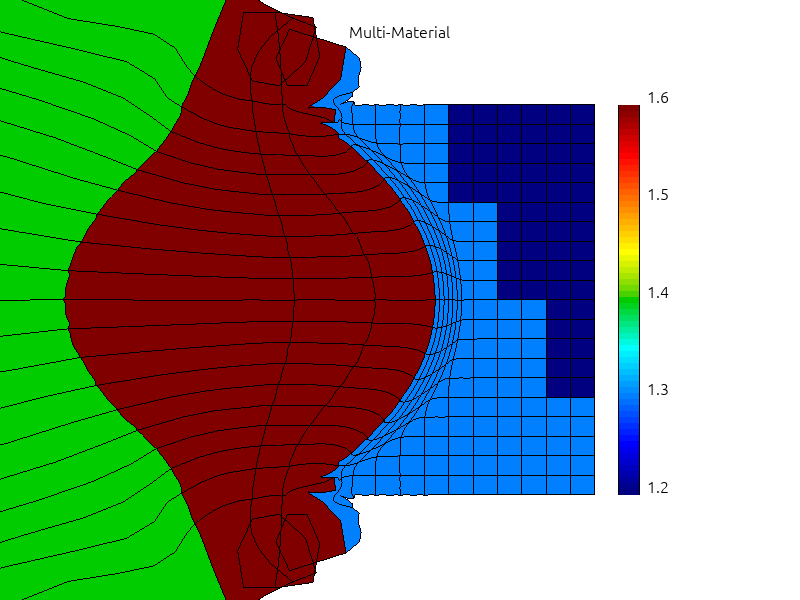
\includegraphics[width=0.3\textwidth]{../figs_NTH/results/OmegaLaser/material_77.png}
	&
	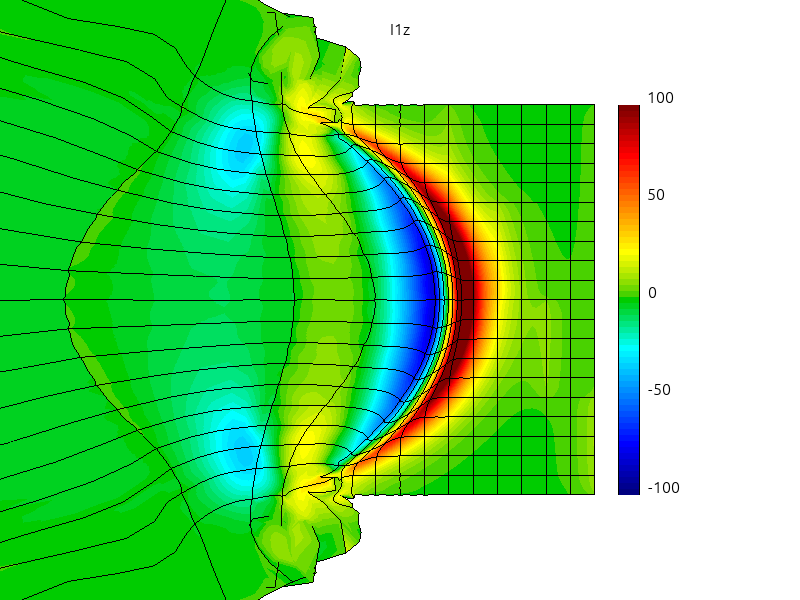
\includegraphics[width=0.3\textwidth]{../figs_NTH/results/OmegaLaser/nonlocalI1z_77.png}
	&
	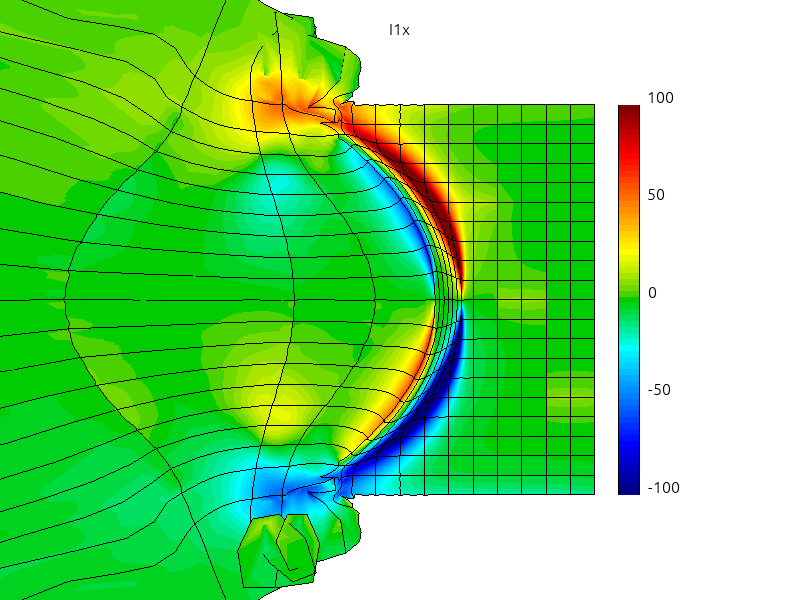
\includegraphics[width=0.3\textwidth]{../figs_NTH/results/OmegaLaser/nonlocalI1x_77.png}
	\end{tabular}
	\end{center}
	\end{figure}
	\begin{tabular}{c}	
	MULTIMAT\\
    SANTA FE, NM, USA\\
	SEPTEMBER 18-22, 2017 
	\end{tabular}
}
%\date{COST Working Group Meeting\\
%Advanced X-ray spatial and temporal metrology\\
%July 9-10, 2015, Madrid}      

\begin{comment} % headline
\defbeamertemplate*{headline}{miniframes theme}%{shadow theme}
{%
  \leavevmode%
  %\hbox{\begin{beamercolorbox}[wd=1.0\paperwidth]{author in head/foot}%
  %  \usebeamerfont{author in head/foot}\insertframenumber\,/\,\inserttotalframenumber\hfill
  %    \includegraphics[width=0.25\textwidth]{../figs/ECOP2_EN.eps} 
  %    \includegraphics[width=0.15\textwidth]{../figs/ELI.eps}
  %    \includegraphics[width=0.2\textwidth]{../figs/FzU.eps}
  %\end{beamercolorbox}}%
  %\hbox{\begin{beamercolorbox}[wd=.35\paperwidth,ht=5.0ex,dp=-1.125ex,leftskip=.3cm plus1fil,rightskip=.3cm]{author in head/foot}%
  %  \usebeamerfont{author in head/foot}\insertframenumber\,/\,\inserttotalframenumber
  %\end{beamercolorbox}%
  %\begin{beamercolorbox}[wd=.65\paperwidth,ht=5.0ex,dp=0.0ex,leftskip=.3cm,rightskip=.3cm plus1fil]{title in head/foot}% 
  %  \usebeamerfont{title in head/foot}
  %    \includegraphics[width=0.22\textwidth]{../figs/ECOP2_EN.eps} 
  %    \includegraphics[width=0.12\textwidth]{../figs/ELI.eps}
  %    \includegraphics[width=0.2\textwidth]{../figs/FzU.eps}    
  %\end{beamercolorbox}}%  
  \hbox{\hfill
      %\includegraphics[width=0.22\textwidth]{../figs/ECOP2_EN.eps} 
	  %\includegraphics[width=0.065\textwidth]{../figs/fjfi_logo.eps}
	  %\includegraphics[width=0.05\textwidth]{../figs/cvut_logo.eps}
      
	  %\includegraphics[width=0.12\textwidth]{../figs/ELI.eps}
      %\includegraphics[width=0.2\textwidth]{../figs/FzU.eps}    
	  %\includegraphics[width=0.15\textwidth]{../figs/logoifn.eps}
	  %\includegraphics[width=0.06\textwidth]{../figs/fjfi_logo.eps}

	  \includegraphics[width=0.08\textwidth]{../figs/ELI.eps}
      \includegraphics[width=0.16\textwidth]{../figs/FzU.eps}    
	  \includegraphics[width=0.11\textwidth]{../figs/logoifn.eps}
	  \includegraphics[width=0.04\textwidth]{../figs/fjfi_logo.eps}  
  }%    
  \vskip0pt%
}
\end{comment} % headline

\defbeamertemplate*{footline}{miniframes theme}%{shadow theme}
{%
  \leavevmode%
  \hbox{\begin{beamercolorbox}[wd=.5\paperwidth,ht=2.5ex,dp=1.125ex,leftskip=.3cm plus1fil,rightskip=.3cm]{author in head/foot}%
    \usebeamerfont{author in head/foot}\insertframenumber\,/\,\inserttotalframenumber\hfill\insertshortauthor
  \end{beamercolorbox}%
  \begin{beamercolorbox}[wd=.5\paperwidth,ht=2.5ex,dp=1.125ex,leftskip=.3cm,rightskip=.3cm plus1fil]{title in head/foot}% 
    \usebeamerfont{title in head/foot}\insertshorttitle% 
  \end{beamercolorbox}}%
  \vskip0pt%
}      
      
\begin{document}
\begin{frame}
 \titlepage
\end{frame}

%\begin{frame}
%\tableofcontents
%\end{frame}

%\section{Introduction to nonlocal transport in laser-heated plasma 
%hydrodynamics}

%\subsection{Nonlocal transport models review}

\newcommand{\edf}{\colorimportant{f}}
\begin{frame}
\begin{center}
{\large Hydrodynamic model of plasma}
\begin{block}{Boltzmann transport equation}
\begin{equation}
  \frac{\partial \edf}{\partial t} + 
  \vect{v}\cdot\nabla_x \edf + \frac{q_e}{m_e}\left(\vect{E}
  +\frac{\vect{v}}{c}\times\vect{B}\right)\cdot
  \nabla_{\vect{v}} \edf 
  = 
  C(\edf, \edf)
  \nonumber
\end{equation}
\end{block}
\begin{block}{Fluid equations}
\begin{eqnarray}
	\frac{\dI \rho}{\dI t} &=& - \rho \nablax\cdot\vect{U}%\, ,
	\label{lagrange_ei_mass_equation} \nonumber\\
	\rho \frac{\dI \vect{U}}{\dI t} 
	&=& \nablax\cdot\matr{\sigma}%\, ,
	\label{lagrange_ei_momentum_equation} \nonumber\\
	\rho\frac{\dI \varepsilon}{\dI t} &=& 
	\matr{\sigma}:\nablax\vect{U}
	- \nablax\cdot\vect{q}%\, ,
	\label{lagrange_i_energy_equation} \nonumber
\end{eqnarray}
\end{block}
\begin{block}{Microscopic closure}
\begin{eqnarray}
	\matr{\sigma} &=& -\rho
	\int (\vect{v}-\vect{U})\otimes
	(\vect{v}-\vect{U})\, \edf\, \dI \vect{v}^3 \approx -\matr{I} p 
	+ \tilde{\matr{\sigma}}(\nabla \vect{U})
	\label{stress_tensor}\nonumber\\
	\vect{q} &=& \frac{\rho}{2} 
	\int |\vect{v} - \vect{U}|^2
	(\vect{v}-\vect{U})\, \edf\, \dI \vect{v}^3 \approx 
	2\pi\rho 
	\int_{4\pi}\vect{n}\int_0^\infty 
	|\vect{v}|^5 \edf\, \dI |\vect{v}|\, \dI \vect{n}
	\approx -\kappa(T^{2.5})\nabla T
	\label{heat_flux_vector} \nonumber
\end{eqnarray}
\end{block}
\end{center}
\end{frame}

\begin{frame}
\begin{center}
{\large Nonlocal vs. diffusive transport models}
\begin{figure}
\begin{center}
\begin{tabular}{cc}
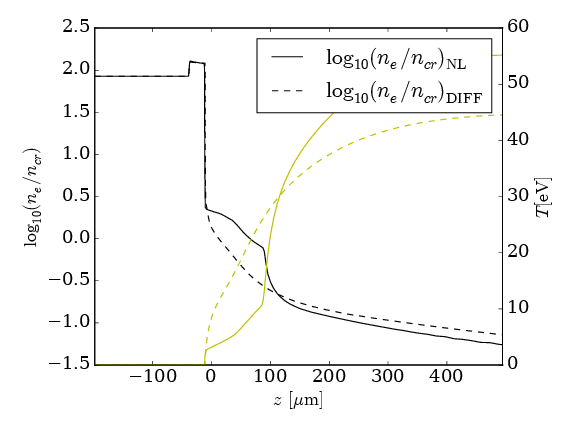
\includegraphics[width=0.4\textwidth]{../figs_NTH/Prepulse/CH_1e22_nencs_Tes.png} 
&
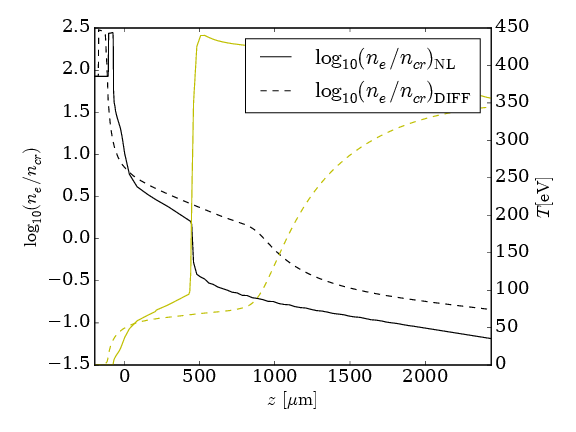
\includegraphics[width=0.4\textwidth]{../figs_NTH/Prepulse/CH_1e24_nencs_Tes.png} 
\\
pre-pulse 10$^{12}$ W/cm$^2$ (10$^{22}$ W/cm$^2$) &
pre-pulse 10$^{14}$ W/cm$^2$ (10$^{24}$ W/cm$^2$)
%\footnote{PIC simulations by Marija Vranic 2017.}
\end{tabular}
%\caption{.}
\label{L4_fig}
\end{center}
\end{figure}

\begin{equation}
  \frac{1}{|\vect{v}|}\frac{\partial f^e}{\partial t} + 
  \vect{n}\cdot\nabla_x f^e + \frac{q_e}{m_e |\vect{v}|}\vect{E}\cdot
  \nabla_{\vect{v}} f^e 
  = 
  \frac{f_{MB}(|\vect{v}|, T_e) - f^e}{\lambda}\, , 
  \nonumber
\end{equation}
%\begin{eqnarray}
%  \frac{1}{\bar{v}}\frac{\partial I^e}{\partial t} + \vect{n}\cdot\nabla I^e 
%  &=& 
%  \frac{\sigma^e T_e - I^e}{\lambda^e}\, , 
%  \nonumber
%  \\
%  \vect{q}_e &=& \int_{4\pi}\vect{n}\, I^e\, \dI\vect{n}\,  ,
%  \nonumber
%\end{eqnarray}
\begin{block}{Chapman-Enskog approximation in small parameter $\lambda$}
\begin{equation}
 f^e = f_0 + \lambda f_1 + O({\lambda}^2) \approx 
 f_{MB}(|\vect{v}|, T_e)
 - f_{MB}(|\vect{v}|, T_e) g(\bar{Z})
   \left(\frac{|\vect{v}|^2}{2 v_{T_e}^2} - 4\right)
    \vect{n}\cdot\frac{\lambda\nabla T_e}{T_e}\nonumber
\end{equation}
%$I \approx \sigma T_e - \lambda \vect{n}\cdot
%  \nabla \left(\sigma T_e\right) + O(\lambda^2)$ 
%$\rightarrow \vect{q} \approx - \lambda \sigma \nabla T_e$ 
\end{block}
\begin{equation}
	\frac{\lambda f_1}{f_0} = 0.25
	\left(\frac{|\vect{v}|^2}{2 v_{T_e}^2} - 4\right)
	\vect{n}\cdot\frac{\lambda(|\vect{v}|)\nabla T_e}{T_e} < 0.1
	\quad\longrightarrow\quad \text{Kn}^e = \frac{\lambda\nabla T_e}{T_e} 
	< 7.5\times10^{-4}
	\nonumber \label{SH_limit}
\end{equation}

\end{center}
\end{frame}


\begin{frame}
\begin{center}
{\Large Nonlocal transport in hydrodynamics review}
\begin{block}{Kinetic Fokker-Planck-Landau equation}
\begin{equation}
  \frac{1}{|\vect{v}|}\frac{\partial f}{\partial t} + 
  \vect{n}\cdot\nabla_x f + \frac{q_e}{m_e}\left(\frac{\vect{E}}{|\vect{v}|}
  +\frac{\vect{n}}{c}\times\vect{B}\right)\cdot
  \nabla_{\vect{v}} f 
  = 
  \frac{1}{\lambda} \nabla_{\vect{v}}\cdot\int 
  \frac{|\vect{v}-\vect{v}'|^2\matr{I} - (\vect{v}-\vect{v}')\otimes 
  \vect{v}-\vect{v}')}{|\vect{v}-\vect{v}'|^3}
  \big(\nabla_{\vect{v}} f(\vect{v}) f(\vect{v}') - 
  f(\vect{v}) \nabla_{\vect{v}} f(\vect{v}')\big) \dI \vect{v}'
  \nonumber
\end{equation}
\end{block}

{\large Computationally efficient simplifications:}
\begin{itemize}
\item \colorimportant{SH flux} electron heat conduction (Chapman-Enskog 
expansion based local approximation [Spitzer and Harm, PR 89, 977 (1953)])
\item \colorimportant{LMV delocalized flux} (1D spatial convolution of SH flux 
[Luciani, Mora, and Virmont, PRL
51, 1664 (1983).], further improved in spectral space 
[Epperlein and Short, PF B 4, 2211
(1992)]
\item \colorimportant{SNB} multi-dimensional extension (linear transport 
equation of SH flux [Schurtz, Nicolai, and Busquet, PoP 7, 4238 (2000)])
\item \colorimportant{M1 model} (finite transport equation moments hierarchy 
based on angular entropy minimization closure [Sorbo et al, PoP 22, 
082706 (2015)])
\item \colorimportant{BGK transport equation} (1D analytic 
solution [Manheimer, Colombant, and Goncharov, PoP 15, 083103 (2008)]) 
\end{itemize}

\begin{block}{Kinetic Nonlocal Transport Hydrodynamic (NTH) equation}
\begin{equation}
  %\frac{1}{|\vect{v}|}\frac{\partial f}{\partial t} + 
  \vect{n}\cdot\nabla_x f + \frac{q_e}{m_e |\vect{v}|}\left(\vect{E}\cdot
  \vect{n}\frac{\partial}{\partial |\vect{v}|}f 
  + \left(\frac{\vect{E}}{|\vect{v}|}+\frac{\vect{n}}{c}\times\vect{B}\right)\cdot\nabla_{\vect{n}} f\right)
  = 
  \frac{f_{MB}(|\vect{v}|, T_e) - f}{\lambda_{ei}} 
  + \frac{|\vect{v}|}{\lambda_{ee}}\frac{\partial}{\partial |\vect{v}|}
  \left(\frac{v_T^2}{|\vect{v}|}\frac{\partial}{\partial |\vect{v}|} + 1\right) 
  \left(f - f_0\right) 
  \nonumber
\end{equation}
\end{block}
\begin{block}{Radiation transport equation}
\begin{equation}
  %\frac{1}{|\vect{v}|}\frac{\partial f}{\partial t} + 
  \vect{n}\cdot\nabla_x I
  = 
  \frac{I_{P} - I}{\lambda} + \frac{I_0 - I}{\tilde{\lambda}}\, ,\qquad 
  I_0 = \frac{1}{4\pi}\int_{4\pi} I\, \dI \vect{n}\, , \qquad 
  \vect{q} = \int_{4\pi} \vect{n} I\, \dI \vect{n}
  \nonumber
\end{equation}
\end{block}
\end{center}
\end{frame}

%\section{High-order discontinuous Galerkin finite element numerical method}
%\subsection{DG-BGK$\&$Ts scheme for nonlocal radiation and electron transport}

\begin{frame}
\begin{center}

\newcommand{\bxi}{\vect{\xi}_t}
\newcommand{\bomegaPhi}{\vect{\omega}_{\Phi}}
\newcommand{\bomegaTheta}{\vect{\omega}_{\Theta}}
\newcommand{\bpsi}{\vect{\psi}_{z}}
\newcommand{\bphi}{\vect{\phi}_{z}}
\newcommand{\Omx}{\Omega_z}
\newcommand{\Gmx}{\Gamma_z}

%\myheading{Finite element discrete variational principle of 
%the axial symmetric BGK transport equation}
\begin{block}{Planar geometry - transport equation}
\begin{equation}
   %\frac{1}{\bar{v}}\frac{\partial \ff}{\partial t} + 
   \cos(\Phi)\frac{\partial \ff}{\partial z} = 
   S_T T_e - k \ff\, ,
   \nonumber %\forall \psi_I\in H\, , \nonumber\label{continuous_DG}
\end{equation}
\end{block}
\begin{equation}
\colorf{
\ff(t, z, \Phi) = 
\left(\bomegaPhi\otimes\bpsi \right)^T\cdot\vect{\ff}^{n+1}
}
, 
\colorTe{
T_e(t, z) = \bphi^T\cdot\vect{T}^{n+1}_e
}
\nonumber
\end{equation}
Composition of the multi-dimensional interpolation based on 
 $\colorimportant{outer product \otimes}$
%, and 
%$T_i(t, \vect{x}) = \left(\bxi\otimes\tilde{\bphi} \right)^T
%\cdot\vect{T}_i$, where the basis functions read
\begin{equation}
\bomegaPhi = [\omega_1(\Phi), .., \omega_{M_\Phi}(\Phi)]^T,
\bpsi = [\psi_1(z), .., \psi_{N_f}(z)]^T,\,
\bphi = [\phi_1(z), .., \phi_{N_e}(z)]^T
%,\, 
%\tilde{\bphi} = [\tilde{\phi}_1(\vect{x}), .., \tilde{\phi}_{N_i}(\vect{x})]^T.
\nonumber
\end{equation} 

\begin{multline}
  \int_{\OPhi} \int_{\Omx} 
  \left(\bomegaPhi\otimes\bpsi\right)\otimes
  %\Bigg[\frac{1}{\bar{v}}\left(\bomegaPhi\otimes\bpsi\right)^T\cdot
  %\frac{\colorf{\vect{\ff}^{n+1}} - \colorf{\vect{\ff}^n}}{\Delta t} \\
  \Bigg[\cos(\Phi) \left(\bomegaPhi\otimes\frac{\partial \bpsi}{\partial z}
  \right)^T\cdot\colorf{\vect{\ff}^{n+1}}
  + k \left(\bomegaPhi\otimes\bpsi \right)^T
  \cdot\colorf{\vect{\ff}^{n+1}}
  -\left(\bomegaPhi\otimes\bphi \right)^T
  \cdot\matr{S}_T\cdot\colorTe{\vect{T_e}^{n+1}}\Bigg]\, 
  \dI \Omx\, \sin(\Phi)\, \dI \Phi =\\
   \int_{\OPhi} \int_{\Gamma_{{\vect{n}\cdot\vect{n}_{\Gamma}<0}}}
   \left(\bomegaPhi\otimes\bpsi\right)\otimes
   \Bigg[\left(\bomegaPhi\otimes\bpsi\right)^T
   \cdot\colorf{\vect{\ff}^{n+1}}-
   \left(\bomegaPhi\otimes\tilde{\bpsi}\right)^T
   \cdot
   \colorimportant{\tilde{\vect{\ff}}}\Bigg]
   \left( \cos(\Phi)\vect{n}_{\Gamma}^z \right)\, 
   \dI \Gmx\, \sin(\Phi)\, \dI \Phi
   %\label{continuous_DG}
   \nonumber
\end{multline} 

\begin{block}{Discrete DG transport equation - transport operator inversion
$\quad\colorf{\vect{\ff}^{n+1} = \matr{A}\cdot\colorTe{\vect{T}^{n+1}_e} + 
\vect{b}(\colorimportant{\tilde{\vect{\ff}}})}$}
\begin{equation}
%\frac{1}{\bar{v}}\matr{M}\cdot
%\frac{\colorf{\vect{\ff}^{n+1}} - \colorf{\vect{\ff}^n}}{\Delta t} +
\matr{D}\cdot\colorf{\vect{\ff}^{n+1}}
+ k \matr{M}
\cdot\colorf{\vect{\ff}^{n+1}}
- \matr{B}\cdot\colorf{\vect{\ff}^{n+1}} = 
\matr{S}\cdot\colorTe{\vect{T_e}^{n+1}}
- \tilde{\matr{B}}\cdot\colorimportant{\tilde{\vect{\ff}}}
\nonumber
\end{equation}
\end{block}

\end{center}
\end{frame}

\begin{frame}
%\mycaptiontable{
\begin{center}
\myheading{Exact steady state "given direction" transport} 
%Photons are generated by the static source 
%function $\sin(\pi\, z)$ and propagate from left to right. 
\begin{equation}
  \cos(\Phi_0)\, \frac{\dI \ff(z, \Phi_0)}{\dI z} = k\, (\sin(\pi z) 
  - \ff(z, \Phi_0))
  %\, . 
  \nonumber \label{slab_I}
\end{equation}
Three different values of $k= 10^{-4}, 1, 10^4$, which corresponds to 
free-streaming, nonlocal, and diffusive transport ($\Phi_0=\pi/4$).
%The normalized exact solution is represented with lines and corresponding 
%numerical approximation with stars. 
%The maximum value of $I$ in case of
%$k= 10^{-4}, 1, 10^4$ are $I_{max}=7.2\cdot10^{-9}, 0.51, 1$, respectively.
%}

%\begin{center}

\begin{tabular}{lc}
\begin{pcolumn}{0.4}
  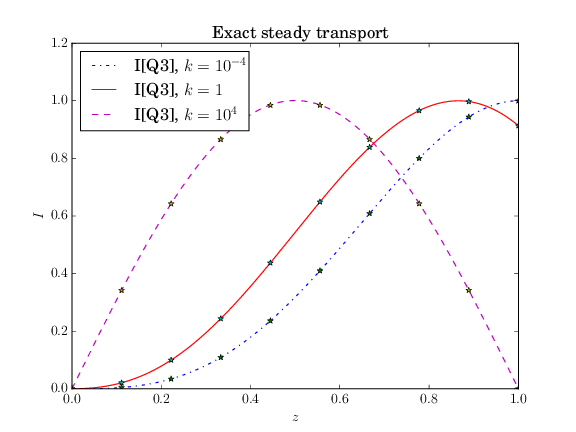
\includegraphics[width=1.1\textwidth]{../figs_NTH/exact_steady_test.png}
  %\mycaptionfig{Nonlocal steady state solution.} 
  %\mycaptionfig{In case of $k=1$ the transport is nonlocal, in case of $k=1\text{e}4$ the transport is diffusive. Opacity $k$ is defined as $k = \lambda^{-1}$.}
\end{pcolumn}& 
\begin{pcolumn}{0.4}
  %\vsp{5}
  \scalebox{0.7}{
\begin{tabular}{|c|c|c|c|c|c|c|c|}
\hline
element & cells & $E^{k=10^{-4}}_{L1}$ & $q^{k=10^{-4}}_{L1}$& $E^{k=1}_{L1}$ & $q^{k=1}_{L1}$& $E^{k=10^4}_{L1}$ & $q^{k=10^4}_{L1}$ \\ 
\hline
I[Q1] & 10 & 2.7e-07 &  & 2.3e-03 &  & 8.3e-03 &  \\ 
\hline
I[Q1] & 20 & 4.9e-08 & 2.5 & 4.3e-04 & 2.4 & 1.6e-03 & 2.4 \\ 
\hline
I[Q1] & 40 & 1.2e-08 & 2.0 & 1.1e-04 & 2.0 & 3.7e-04 & 2.1 \\ 
\hline
I[Q1] & 80 & 2.9e-09 & 2.0 & 2.6e-05 & 2.0 & 9.0e-05 & 2.1 \\ 
\hline
\hline
I[Q2] & 10 & 4.6e-09 &  & 4.1e-05 &  & 3.5e-07 &  \\ 
\hline
I[Q2] & 20 & 4.1e-10 & 3.5 & 3.5e-06 & 3.5 & 5.2e-08 & 2.8 \\ 
\hline
I[Q2] & 40 & 4.5e-11 & 3.2 & 4.0e-07 & 3.2 & 1.2e-08 & 2.1 \\ 
\hline
I[Q2] & 80 & 5.4e-12 & 3.1 & 4.7e-08 & 3.1 & 2.8e-09 & 2.1 \\ 
\hline
\hline
I[Q3] & 10 & 7.3e-11 &  & 2.6e-07 &  & 2.3e-06 &  \\ 
\hline
I[Q3] & 20 & 2.8e-12 & 4.7 & 8.4e-09 & 5.0 & 1.0e-07 & 4.5 \\ 
\hline
I[Q3] & 40 & 1.5e-13 & 4.2 & 4.3e-10 & 4.3 & 5.6e-09 & 4.2 \\ 
\hline
I[Q3] & 80 & 8.9e-15 & 4.1 & 2.4e-11 & 4.1 & 3.3e-10 & 4.1 \\ 
\hline
%\hline
\end{tabular}
	}
\end{pcolumn}
\end{tabular}

It is worth mentioning that the method works well also in diffusive 
limit $k=10^4$ ($Kn \approx 10^{-4}$).
\end{center}
\end{frame}

\begin{frame}
%\mycaptiontable{
\begin{center}
\myheading{Exact steady state "full" transport} 

\begin{tabular}{ll}
\begin{pcolumn}{0.42}
%\scalebox{0.8}{
%\begin{tabular}{c}
Model steady equation
\begin{equation}
  \cos(\Phi)\, \frac{\dI \ff(z, \Phi)}{\dI z} = 
  k\, (S(z) - \ff(z, \Phi))
  %\, , \quad S(z) = a\, (1 - \cos(z))\, .
  \nonumber \label{slab_I}
\end{equation}
$ $
%\\
Energy density flux
\begin{equation}
	\vect{q}(z) = 2\pi \int_0^\pi \cos(\Phi)\, \ff(z, \Phi)\, \sin(\Phi)\, 
	\dI \Phi 
	\nonumber \label{slab_I}
\end{equation} 
%\\
\colorimportant{Divergence of energy density flux}
\begin{equation}
	\colorimportant{\nabla\cdot\vect{q}(z) = 2\pi \int_0^\pi \cos(\Phi)\, 
	\frac{\partial \ff(z, \Phi)}{\partial z}\, \sin(\Phi)\, \dI \Phi} 
	\nonumber \label{slab_I}
\end{equation}
%\end{tabular}
%}
\end{pcolumn} &

\begin{pcolumn}{0.5}
  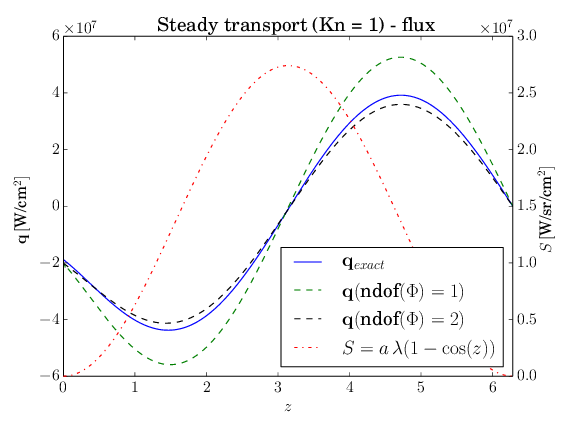
\includegraphics[width=1.0\textwidth]{../figs_NTH/steady_cosine_flux.png}
  %\mycaptionfig{Nonlocal steady state solution.} 
  %\mycaptionfig{In case of $k=1$ the transport is nonlocal, in case of $k=1\text{e}4$ the transport is diffusive. Opacity $k$ is defined as $k = \lambda^{-1}$.}
\end{pcolumn}
\end{tabular}

\begin{pcolumn}{1.0}
  %\vsp{5}
 Relative L1 error convergence in polar angle $\Phi$ of 
$\colorimportant{\nabla\cdot\vect{q}}$
  \scalebox{0.8}{
\begin{tabular}{|c|c|c|c|c|c|c|c|c|}
\hline
 transport regime & Kn=$\lambda/L$ | ndof($\Phi$) & 1 & 2 & 3 & 4 & 5 & 20 & 40  \\ 
\hline
 transparent/ballistic & 100.0 & 1.5e-01 & 4.1e-01 & 9.5e-02 & 2.4e-01 & 
 7.1e-02 & 5.1e-02 & 2.2e-02
\\ 
\hline
 nonlocal/highly anisotropic & 10.0 & 2.0e-01 & 3.7e-01 & 1.1e-01 & 2.0e-01 & 
 7.8e-02 & 1.3e-02 & 1.1e-03 
\\ 
\hline
 nonlocal/anisotropic & 1.0 & 3.5e-01 & 8.8e-02 & 2.6e-02 & 1.1e-02 & 2.7e-03 & 
 1.1e-05 & 9.6e-07
\\ 
\hline
 nonlocal/almost isotropic & 0.1 & 1.5e-01 & 9.6e-03 & 4.8e-03 & 3.3e-3 & 
 6.9e-04 & 5.7e-07 & 4.6e-07 
\\ 
\hline
 diffusive/isotropic & 0.01 & 1.4e-01 & 1.0e-02 & 5.9e-03 & 4.5e-03 & 2.0e-03 &
 2.9e-05 & 2.9e-05
\\ 
\hline
%\hline
\end{tabular}
}
\end{pcolumn}
\end{center}
\end{frame}

\begin{frame}
\begin{center}

\newcommand{\bxi}{\vect{\xi}_t}
\newcommand{\bomegaPhi}{\vect{\omega}_{\Phi}}
\newcommand{\bomegaTheta}{\vect{\omega}_{\Theta}}
\newcommand{\bpsi}{\vect{\psi}_{z}}
\newcommand{\bphi}{\vect{\phi}_{z}}
\newcommand{\Omx}{\Omega_z}
\newcommand{\Gmx}{\Gamma_z}

%\myheading{Finite element discrete variational principle of 
%the axial symmetric BGK transport equation}
\begin{block}{Planar geometry - transport equation}
\begin{equation}
   %\frac{1}{\bar{v}}\frac{\partial \ff}{\partial t} + 
   \cos(\Phi)\frac{\partial \ff}{\partial z} = 
   S_T T_e - (k + \cos(\Phi) E_z) \ff + \sigma I_0\, ,
   \quad I_0 = \frac{1}{2}\int_{\OPhi} I \sin(\Phi)\, \dI \Phi
   \nonumber %\forall \psi_I\in H\, , \nonumber\label{continuous_DG}
\end{equation}
\end{block}
\begin{equation}
\colorf{
\ff(t, z, \Phi) = 
\left(\bomegaPhi\otimes\bpsi \right)^T\cdot\vect{\ff}^{n+1}
}
, 
\colorTe{
T_e(t, z) = \bphi^T\cdot\vect{T}^{n+1}_e
}
\nonumber
\end{equation}
Composition of the multi-dimensional interpolation based on 
 $\colorimportant{outer product \otimes}$
%, and 
%$T_i(t, \vect{x}) = \left(\bxi\otimes\tilde{\bphi} \right)^T
%\cdot\vect{T}_i$, where the basis functions read
\begin{equation}
\bomegaPhi = [\omega_1(\Phi), .., \omega_{M_\Phi}(\Phi)]^T,
\bpsi = [\psi_1(z), .., \psi_{N_f}(z)]^T,\,
\bphi = [\phi_1(z), .., \phi_{N_e}(z)]^T
%,\, 
%\tilde{\bphi} = [\tilde{\phi}_1(\vect{x}), .., \tilde{\phi}_{N_i}(\vect{x})]^T.
\nonumber
\end{equation} 

\begin{multline}
  \int_{\OPhi} \int_{\Omx} 
  \left(\bomegaPhi\otimes\bpsi\right)\otimes
  %\Bigg[\frac{1}{\bar{v}}\left(\bomegaPhi\otimes\bpsi\right)^T\cdot
  %\frac{\colorf{\vect{\ff}^{n+1}} - \colorf{\vect{\ff}^n}}{\Delta t} \\
  \Bigg[\cos(\Phi) \left(\bomegaPhi\otimes\frac{\partial \bpsi}{\partial z}
  \right)^T\cdot\colorf{\vect{\ff}^{n+1}}
  + (k + \cos(\Phi) E_z) \left(\bomegaPhi\otimes\bpsi \right)^T
  \cdot\colorf{\vect{\ff}^{n+1}}
  - \frac{\sigma}{2} \int_{\OPhi}\bomegaPhi^T \sin(\Phi)\dI\Phi \otimes\bpsi^T
  \cdot\colorf{\vect{\ff}^{n+1}}\\
  -\left(\bomegaPhi\otimes\bphi \right)^T
  \cdot\matr{S}_T\cdot\colorTe{\vect{T_e}^{n+1}}\Bigg]\, 
  \dI \Omx\, \sin(\Phi)\, \dI \Phi =\\
   \int_{\OPhi} \int_{\Gamma_{{\vect{n}\cdot\vect{n}_{\Gamma}<0}}}
   \left(\bomegaPhi\otimes\bpsi\right)\otimes
   \Bigg[\left(\bomegaPhi\otimes\bpsi\right)^T
   \cdot\colorf{\vect{\ff}^{n+1}}-
   \left(\bomegaPhi\otimes\tilde{\bpsi}\right)^T
   \cdot
   \colorimportant{\tilde{\vect{\ff}}}\Bigg]
   \left( \cos(\Phi)\vect{n}_{\Gamma}^z \right)\, 
   \dI \Gmx\, \sin(\Phi)\, \dI \Phi
   %\label{continuous_DG}
   \nonumber
\end{multline} 

\begin{block}{Discrete DG transport equation - transport operator inversion
$\quad\colorf{\vect{\ff}^{n+1} = \matr{A}\cdot\colorTe{\vect{T}^{n+1}_e} + 
\vect{b}(\colorimportant{\tilde{\vect{\ff}}})}$}
\begin{equation}
%\frac{1}{\bar{v}}\matr{M}\cdot
%\frac{\colorf{\vect{\ff}^{n+1}} - \colorf{\vect{\ff}^n}}{\Delta t} +
\matr{D}\cdot\colorf{\vect{\ff}^{n+1}}
+ \left((k + \sigma) \matr{M} + E_z \matr{M}_{\cos(\Phi)} 
- \sigma \matr{MI}\right)
\cdot\colorf{\vect{\ff}^{n+1}}
- \matr{B}\cdot\colorf{\vect{\ff}^{n+1}} = 
\matr{S}\cdot\colorTe{\vect{T_e}^{n+1}}
- \tilde{\matr{B}}\cdot\colorimportant{\tilde{\vect{\ff}}}
\nonumber
\end{equation}
\end{block}

\end{center}
\end{frame}

\begin{frame}

\newcommand{\bxi}{\vect{\xi}_t}
\newcommand{\bomegaPhi}{\vect{\omega}_{\Phi}}
\newcommand{\bomegaTheta}{\vect{\omega}_{\Theta}}
\newcommand{\bpsi}{\vect{\psi}_{z}}
\newcommand{\bphi}{\vect{\phi}_{z}}
\newcommand{\Omx}{\Omega_z}

%The unknowns are discretized as finite element interpolations, i.e. 
%$\colorimportant{f(t, \vect{x}, \vartheta) = 
%\left(\bxi\otimes\bomega\otimes\bpsi \right)^T
%\cdot\vect{f}}$, $\colorimportant{T_e(t, \vect{x}) = 
%\left(\bxi\otimes\bpsi \right)^T
%\cdot\vect{T}_e}$, and 
%$T_i(t, \vect{x}) = \left(\bxi\otimes\tilde{\bpsi} \right)^T
%\cdot\vect{T}_i$, where the basis functions read

%\myheading{Finite element discrete variational principle of 
%the axial symmetric BGK transport equation}
\begin{block}{Planar geometry - energy equation equipped with the 
\colorimportant{nonlocal transport}}
\begin{equation}
   a\frac{\dI T_e}{\dI t} + G_{ei} (T_e-T_i) + \int_{4\pi}
   %\left( \frac{1}{\bar{v}}\frac{\partial \ff}{\partial t} + 
   \colorimportant{\cos(\Phi)\frac{\partial \ff}{\partial z}} 
   %\right) 
   \sin(\Phi)\, \dI \Phi\, \dI \Theta
   = P_e  
   \nonumber %\forall \psi_I\in H\, , \nonumber\label{continuous_DG}
\end{equation}
\end{block}
 
\begin{equation}
\colorf{
\ff(t, z, \Phi) = 
\left(\bomegaPhi\otimes\bpsi \right)^T\cdot\vect{\ff}^{n+1}
}
, 
\colorTe{
T_e(t, z) = \bphi^T\cdot\vect{T}^{n+1}_e
}
, 
\colorTi{
T_i(t, z) = \tilde{\bphi}^T\cdot\vect{T}^{n+1}_i
}
\nonumber
\end{equation}
\begin{multline}
   \int_{\Omx} 
   \bphi\otimes
   \Bigg[a\, \bphi^T
   \cdot\frac{\colorTe{\vect{T}^{n+1}_e}- \colorTe{\vect{T}^{n}_e}}{\Delta t} + 
   G_{ei} \left(\bphi^T\cdot\colorTe{\vect{T}^{n+1}_e} 
   - \tilde{\bphi}^T\cdot\colorTi{\vect{T}^{n+1}_i}\right) +  
   2 \pi \int_{\OPhi}
   %\Bigg(\frac{1}{\bar{v}}\left(\bomegaPhi\otimes\bpsi\right)^T\cdot
   %\frac{\colorf{\vect{\ff}^{n+1}} - \colorf{\vect{\ff}^{n}}}{\Delta t} +
   \cos(\Phi) \left(\bomegaPhi\otimes\frac{\partial \bpsi}{\partial z}
   \right)^T\cdot\colorf{\vect{\ff}^{n+1}} 
   %\Bigg) 
   \sin(\Phi)\, 
   \dI \Phi \\
   - \bphi^T\cdot\vect{P}_e
   \Bigg] \dI \Omx =  \vect{0}\, .
   %\label{DGBGK_DG_temperature_equation}    
   \nonumber
\end{multline}

\begin{equation}
a \matr{M}\cdot
\frac{\colorTe{\vect{T}^{n+1}_e}- \colorTe{\vect{T}^{n}_e}}{\Delta t}
+ \matr{G}_{ei}\cdot\colorTe{\vect{T}^{n+1}_e}
- \tilde{\matr{G}}_{ei}\cdot\colorTi{\vect{T}^{n+1}_i}
%+ \frac{1}{\bar{v}}\matr{MI}\cdot
%\frac{\colorf{\vect{\ff}^{n+1}} - \colorf{\vect{\ff}^n}}{\Delta t}
+ \matr{DI}\cdot\colorf{\vect{\ff}^{n+1}}
 = 
\vect{P}_e
\nonumber
\end{equation}

\begin{pcolumn}{1.}
\begin{block}{\centering \colorimportant{DG-BGK$\&$Ts} scheme, where  
	$\colorf{\vect{\ff}^{n+1}=\matr{A}}\cdot\colorTe{\vect{T}_e^{n+1}}
	\colorf{+ \vect{b}}$}
\begin{equation}
\matr{A}_{T_e}(\colorf{\matr{A}})\cdot\colorTe{\vect{T}^{n+1}_e} 
+ \tilde{\matr{G}}_{ei}\cdot\colorTi{\vect{T}^{n+1}_i} = 
\vect{b}_{T_e}(\colorf{\vect{b}}) 
\nonumber \label{DGBGKT}
\end{equation}
\end{block}
\footnote{[Holec et al, IJNMF 83, 779 (2017)]}
\end{pcolumn}

%\begin{tabular}{l}
%\hline
%Entire algebraic construction of DG-BGK$\&$Ts is based on 
%\colorimportant{mfem.org}
%\end{tabular}

\end{frame}

%\subsection{Approximate multi-group diffusion test}
\begin{frame}
\begin{center}
\myheading{Approximate multi-group diffusion test}

\begin{tabular}{ll}

\begin{pcolumn}{0.45}
%\scalebox{0.8}{
%\begin{tabular}{c}
Two energy groups transport model
\begin{equation}
  %\frac{1}{c_\pp}\frac{\partial \ff_{g_j}}{\partial t} + 
  \cos(\Phi)\, 
  \frac{\partial \ff_{g_j}}{\partial z} 
  = 
  k_{g_j}\, (S_T T - \ff_{g_j})
  \nonumber \label{slab_I}
\end{equation}
%  \\
\begin{equation}
  a\, \frac{\partial T}{\partial t} 
  =
  - \sum_{j=1, 2}
  \frac{2\pi}{\Delta_{g_j}} \int_0^\pi
   %\left( 
   %\frac{1}{c_\pp}\frac{\partial \ff_{g_j}}{\partial t} + 
   \cos(\Phi)\frac{\partial \ff_{g_j}}{\partial z} 
   %\right) 
   \sin(\Phi)\, \dI \Phi\,\, , 
   \nonumber\label{PTE_temperature_equation} 
\end{equation}
%\\
%\end{tabular}
%}
\end{pcolumn} &

\begin{pcolumn}{0.5}
  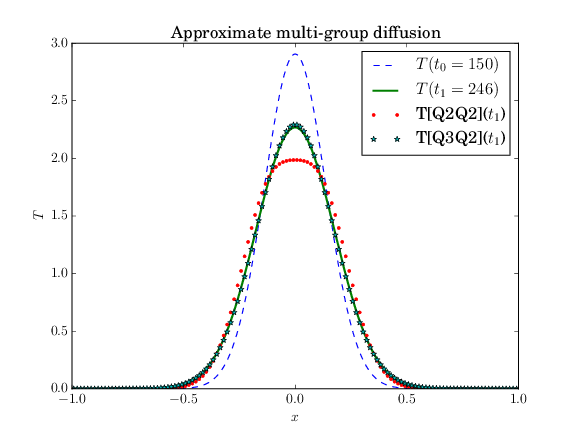
\includegraphics[width=0.9\textwidth]{../figs_NTH/approximate_diffusion_test.png}
  %\mycaptionfig{Nonlocal steady state solution.} 
  %\mycaptionfig{In case of $k=1$ the transport is nonlocal, in case of $k=1\text{e}4$ the transport is diffusive. Opacity $k$ is defined as $k = \lambda^{-1}$.}
\end{pcolumn}

\end{tabular}

Diffusive(\colorimportant{local}) asymptotic behavior of the two energy 
groups transport model
\begin{equation}
  \colorimportant{
  \ff_{g_j} \approx S_T \left( T 
  - \frac{\cos(\Phi)}{k_{g_j}}\frac{\partial T}{\partial z} \right)
  \xrightarrow{local}
  %\left(
  a 
  %+ 4\pi\sigma\left( \frac{1}{\Delta_{g_1}} +
  %\frac{1}{\Delta_{g_2}} \right) \right) 
  \frac{\partial T}{\partial t} 
  \approx
  \frac{4\pi S_T}{3}\left( \frac{1}{k_{g_1}\Delta_{g_1}} +
  \frac{1}{k_{g_2}\Delta_{g_2}} \right) \frac{\partial^2 T}{\partial z^2}
  }
   \, .
   \nonumber\label{PTE_temperature_equation} 
\end{equation}

\begin{pcolumn}{1.0}

\scalebox{0.8}{
\begin{tabular}{|c|c|c|c|c|c|}
\hline
cells & 32 & 64 & 128 & 256 & 512 \\ 
\hline
T[Q1Q1]& 2.2e-01 [5]& 2.4e-01 (-0.1)& 2.3e-01 (0.0)& 2.3e-01 (0.0)& 2.3e-01 (0.0)\\ 
\hline
T[Q2Q2]& 8.7e-02 [4]& 9.5e-02 (-0.1)& 9.8e-02 (-0.0)& 9.6e-02 (0.0)& 9.1e-02 (0.1)\\ 
\hline
T[Q3Q2]& 1.2e-01 [4]& 5.7e-02 (1.1)& 1.0e-02 (2.5)& 1.3e-03 (2.9)& --\\ 
\hline
T[Q3Q3]& 7.6e-02 [4]& 4.6e-02 (0.7)& 9.8e-03 (2.2)& 1.3e-03 (2.9)& --\\ 
\hline
T[Q4Q4]& 2.9e-02 [4]& 9.6e-03 (1.6)& 1.3e-03 (2.9)& --& --\\ 
\hline
T[Q5Q5]& 2.3e-03 [4]& 8.2e-05 (4.8)& --& --& --\\ 
\hline
T[Q6Q6]& 1.7e-04 [4]& --& --& --& --\\ 
\hline
\end{tabular}
}
\end{pcolumn}

\end{center}
\end{frame}

%\begin{comment} % RT pics
\newcommand{\RThscale}{0.9}
\begin{frame}
\begin{center}
%{\large Lagrangian High-Order Curvilinear Framework}

 %New generation high-order curvilinear hydrodynamic code
\begin{tabular}{cc}
 \begin{pcolumn}{0.5}
 \begin{varblock}[0.85\textwidth]{Lagrangian High-Order Curvilinear Framework}
 %High-order finite element discretization introduced by 
 %Dobrev, Kolev, and Rieben 
 %
 %Semidiscrete formulation of Euler's equations in Lagrangian frame, 
 %i.e. momentum, energy, and mass conservation, respectively.
 \begin{eqnarray}
   \matr{M}_{\vect{v}}\cdot\frac{\dI \vect{v}}{\dI t} &=& 
     - \matr{F}\cdot\matr{I} \nonumber \\
   \matr{M}_{e}\cdot\frac{\dI \vect{e}}{\dI t} &=& \matr{F}^T\cdot\vect{v} 
     \nonumber \\
   \frac{\dI \vect{x}}{\dI t} &=& \vect{v} \nonumber \\
   \nonumber 
 \end{eqnarray} 
 [Dobrev, Kolev, Rieben, SIAM JSC 34, B606 (2012)]
 \end{varblock}
 \begin{eqnarray}
   \nonumber  
   \\\nonumber\\\nonumber\\\nonumber\\\nonumber\\\nonumber\\\nonumber
   \\\nonumber\\\nonumber\\\nonumber\\\nonumber\\\nonumber\\\nonumber
   \\\nonumber\\\nonumber\\\nonumber\\\nonumber\\\nonumber\\\nonumber
   %\\\nonumber\\\nonumber\\\nonumber\\\nonumber\\\nonumber\\\nonumber
 \end{eqnarray} 
 \end{pcolumn} &
 \includegraphics<1>[height=\RThscale\textheight]{../figs_NTH/RT_figs/merged_GLVis_s01.png}
 \includegraphics<2>[height=\RThscale\textheight]{../figs_NTH/RT_figs/merged_GLVis_s20.png}
 \includegraphics<3>[height=\RThscale\textheight]{../figs_NTH/RT_figs/merged_GLVis_s40.png}
 \includegraphics<4>[height=\RThscale\textheight]{../figs_NTH/RT_figs/merged_GLVis_s59.png}
\end{tabular}
 %\includegraphics<1>[height=\hscale\textheight]{../RT_figs/merged_GLVis_s01.png}
 %\includegraphics<2>[height=\hscale\textheight]{../RT_figs/merged_GLVis_s10.png}
 %\includegraphics<3>[height=\hscale\textheight]{../RT_figs/merged_GLVis_s20.png}
 %\includegraphics<4>[height=\hscale\textheight]{../RT_figs/merged_GLVis_s30.png}
 %\includegraphics<5>[height=\hscale\textheight]{../RT_figs/merged_GLVis_s40.png}
 %\includegraphics<6>[height=\hscale\textheight]{../RT_figs/merged_GLVis_s50.png}
 %\includegraphics<7>[height=\hscale\textheight]{../RT_figs/merged_GLVis_s60.png}
 %\includegraphics<8>[height=\hscale\textheight]{../RT_figs/merged_GLVis_s70.png}
 %\includegraphics<9>[height=\hscale\textheight]{../RT_figs/merged_GLVis_s79.png}
\end{center}
\end{frame}

\begin{frame}
\begin{center}
%{\large Lagrangian High-Order Curvilinear Framework}
 \begin{varblock}[1.0\textwidth]{Nonlocal Extension of Lagrangian High-Order Curvilinear Framework}
 %High-order finite element discretization introduced by 
 %Dobrev, Kolev, and Rieben 
 %
 %Semidiscrete formulation of Euler's equations in Lagrangian frame, 
 %i.e. momentum, energy, and mass conservation, respectively.
 \begin{eqnarray}
   \matr{M}_{\vect{v}}\cdot\frac{\dI \vect{v}}{\dI t} &=& 
     - \matr{F}\cdot\matr{I}\nonumber\\
   k_B \matr{M}_{e}\cdot\frac{\dI \vect{T}}{\dI t} &=& \matr{F}^T\cdot\vect{v}
   - \int_{4\pi} \matr{D}\cdot\vect{I}\, \dI \vect{n}\nonumber \\ 
   \frac{\dI \vect{x}}{\dI t} &=& \vect{v} \nonumber \\
   \matr{D}\cdot\vect{I} &=& \matr{S}\cdot\vect{T} 
   - \left((k+\sigma) \matr{M} + \vect{E}\cdot\matr{M}_{\vect{n}} 
   - \sigma\matr{MI}\right) \cdot\vect{I} + \matr{B}\cdot\vect{I} 
   - \tilde{\matr{B}}\cdot\tilde{\vect{I}} 
   \nonumber 
   \\ \nonumber 
 \end{eqnarray}
\end{varblock}
\begin{tabular}{ccc}
 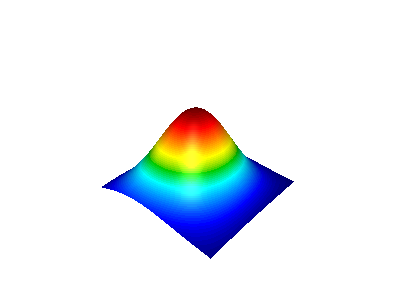
\includegraphics[width=0.4\textwidth]{../figs_NTH/results/triplepoint/nonlocalS.png} 
 &
 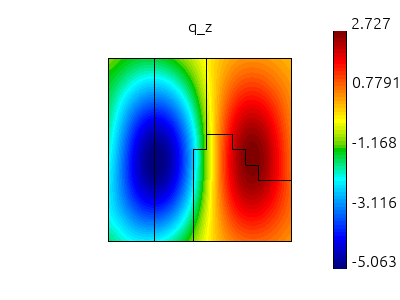
\includegraphics[width=0.28\textwidth]{../figs_NTH/results/triplepoint/nonlocalI1z_0.png}
 &
 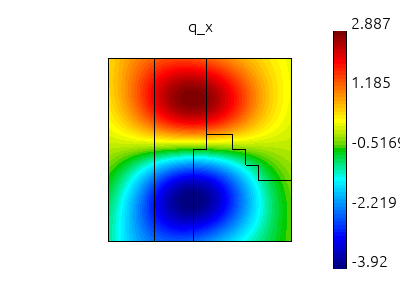
\includegraphics[width=0.28\textwidth]{../figs_NTH/results/triplepoint/nonlocalI1x_0.png}\\
 source $\sin(z)\sin(x)$ & z flux component & x flux component
\end{tabular}
\end{center}
\end{frame}

\begin{frame}
\begin{center}
\begin{tabular}{cc}
 \includegraphics<1>[height=\hscale\textheight]{../figs_NTH/results/triplepoint/temperature_0.png} 
 &
 \includegraphics<1>[height=\hscale\textheight]{../figs_NTH/results/triplepoint/nonlocalI1z_0.png}
 \\
 \includegraphics<1>[height=\hscale\textheight]{../figs_NTH/results/triplepoint/nonlocalI0_0.png} 
 &
 \includegraphics<1>[height=\hscale\textheight]{../figs_NTH/results/triplepoint/nonlocalI1x_0.png}
\end{tabular}
\begin{tabular}{cc}
 \includegraphics<2>[height=\hscale\textheight]{../figs_NTH/results/triplepoint/temperature_17.png} 
 &
 \includegraphics<2>[height=\hscale\textheight]{../figs_NTH/results/triplepoint/nonlocalI1z_17.png}
 \\
 \includegraphics<2>[height=\hscale\textheight]{../figs_NTH/results/triplepoint/nonlocalI0_17.png} 
 &
 \includegraphics<2>[height=\hscale\textheight]{../figs_NTH/results/triplepoint/nonlocalI1x_17.png}
\end{tabular}
\begin{tabular}{cc}
 \includegraphics<3>[height=\hscale\textheight]{../figs_NTH/results/triplepoint/temperature_27.png} 
 &
 \includegraphics<3>[height=\hscale\textheight]{../figs_NTH/results/triplepoint/nonlocalI1z_27.png}
 \\
 \includegraphics<3>[height=\hscale\textheight]{../figs_NTH/results/triplepoint/nonlocalI0_27.png} 
 &
 \includegraphics<3>[height=\hscale\textheight]{../figs_NTH/results/triplepoint/nonlocalI1x_27.png}
\end{tabular}
\begin{tabular}{cc}
 \includegraphics<4>[height=\hscale\textheight]{../figs_NTH/results/triplepoint/temperature_37.png} 
 &
 \includegraphics<4>[height=\hscale\textheight]{../figs_NTH/results/triplepoint/nonlocalI1z_37.png}
 \\
 \includegraphics<4>[height=\hscale\textheight]{../figs_NTH/results/triplepoint/nonlocalI0_37.png} 
 &
 \includegraphics<4>[height=\hscale\textheight]{../figs_NTH/results/triplepoint/nonlocalI1x_37.png}
\end{tabular}
\begin{tabular}{cc}
 \includegraphics<5>[height=\hscale\textheight]{../figs_NTH/results/triplepoint/temperature_47.png} 
 &
 \includegraphics<5>[height=\hscale\textheight]{../figs_NTH/results/triplepoint/nonlocalI1z_47.png}
 \\
 \includegraphics<5>[height=\hscale\textheight]{../figs_NTH/results/triplepoint/nonlocalI0_47.png} 
 &
 \includegraphics<5>[height=\hscale\textheight]{../figs_NTH/results/triplepoint/nonlocalI1x_47.png}
\end{tabular}
\begin{tabular}{cc}
 \includegraphics<6>[height=\hscale\textheight]{../figs_NTH/results/triplepoint/temperature_57.png} 
 &
 \includegraphics<6>[height=\hscale\textheight]{../figs_NTH/results/triplepoint/nonlocalI1z_57.png}
 \\
 \includegraphics<6>[height=\hscale\textheight]{../figs_NTH/results/triplepoint/nonlocalI0_57.png} 
 &
 \includegraphics<6>[height=\hscale\textheight]{../figs_NTH/results/triplepoint/nonlocalI1x_57.png}
\end{tabular}
\begin{tabular}{cc}
 \includegraphics<7>[height=\hscale\textheight]{../figs_NTH/results/triplepoint/temperature_67.png} 
 &
 \includegraphics<7>[height=\hscale\textheight]{../figs_NTH/results/triplepoint/nonlocalI1z_67.png}
 \\
 \includegraphics<7>[height=\hscale\textheight]{../figs_NTH/results/triplepoint/nonlocalI0_67.png} 
 &
 \includegraphics<7>[height=\hscale\textheight]{../figs_NTH/results/triplepoint/nonlocalI1x_67.png}
\end{tabular}
\begin{tabular}{cc}
 \includegraphics<8>[height=\hscale\textheight]{../figs_NTH/results/triplepoint/temperature_womesh_67.png} 
 &
 \includegraphics<8>[height=\hscale\textheight]{../figs_NTH/results/triplepoint/nonlocalI1z_womesh_67.png}
 \\
 \includegraphics<8>[height=\hscale\textheight]{../figs_NTH/results/triplepoint/nonlocalI0_womesh_67.png} 
 &
 \includegraphics<8>[height=\hscale\textheight]{../figs_NTH/results/triplepoint/nonlocalI1x_womesh_67.png}
\end{tabular}
\end{center}
\end{frame}

\begin{frame}
\begin{center}
{\large Curvilinear Framework of Nonlocal Transport}
\begin{block}{Axisymmetric transport equation}
\begin{eqnarray} 
  \sin(\phi) \left(\cos(\theta)\frac{\partial I}{\partial r} 
  - \frac{\sin(\theta)}{r}\frac{\partial I}{\partial \theta}\right) 
  + \cos(\phi)\frac{\partial I}{\partial z} 
  %+ \frac{\vect{n}}{c}\times\vect{B}\cdot\nabla_{\vect{n}} f 
  &=& 
  S_T\, T_e - \left(k + \sigma 
  - \sin(\phi)\cos(\theta) E_r - \cos(\phi) E_z\right) I + \sigma I_0%\, , 
	\label{ap_DGBGK_axissymmetric_transfer_equation}\nonumber\\
   \matr{D}\cdot\vect{I} &=& \matr{S}\cdot\vect{T} 
   - \left((k+\sigma) \matr{M} + \vect{E}\cdot\matr{M}_{\vect{n}} 
   - \sigma\matr{MI}\right) \cdot\vect{I} + \matr{B}\cdot\vect{I} 
   - \tilde{\matr{B}}\cdot\tilde{\vect{I}}\nonumber
\end{eqnarray}
\end{block}\footnote{\colorimportant{{\large mfem.org} -- "My finite element library is higher order than yours..."}}
\begin{itemize}
  \item high-order curvilinear divergence matrix 
\begin{multline}
	\matr{D} = 
	\int_{0}^{\pi}\int_{0}^{\pi} 
	\int_{\Omega} 
	\left(\vect{\omega}_{\theta}\otimes\vect{\omega}_{\phi}
	\otimes\vect{\psi}\right)\otimes\\
	\left( 
	\sin(\phi)\, \vect{\omega}_{\phi}\otimes
	\left(\cos(\theta)\, \vect{\omega}_{\theta}^T\otimes
	\frac{\partial \vect{\psi}^T}{\partial r} 
  - \frac{\sin(\theta)}{r}
  \frac{\partial \vect{\omega}_{\theta}^T}{\partial \theta}\otimes\vect{\psi}^T\right) 
  + \vect{\omega}_{\theta}^T\otimes\cos(\phi)\, \vect{\omega}_{\phi}^T\otimes
  \frac{\partial \vect{\psi}^T}{\partial z} 
	\right)
	r\, \sin(\phi)\dI \Omega \dI\phi\dI\theta \nonumber 
\end{multline}
  \item high-order curvilinear numerical flux matrix
\begin{equation}
	\matr{B} = 
	\int_{0}^{\pi}\int_{0}^{\pi} 
	\int_{\Gamma_{\vect{n}\cdot\vect{n}_{\Gamma}<0}} 
	\left(\vect{\omega}_{\theta}\otimes\vect{\omega}_{\phi}
	\otimes\vect{\psi}\right)\otimes
	\left(\vect{\omega}_{\theta}\otimes\vect{\omega}_{\phi}
	\otimes\vect{\psi}\right)^T 
	\left(\sin(\phi)\cos(\theta) n_{\Gamma_r} + \cos(\phi) n_{\Gamma_z} \right)
	r\, \sin(\phi)\dI \Gamma\dI\phi\dI\theta \nonumber 
\end{equation}
\item proper treatment of Lorentz force
\begin{equation}
 \vect{E}\cdot\vect{n}\frac{\partial I}{\partial |\vect{v}|} + 
 \left(\vect{E}+\vect{n}\times\vect{B}\right)\cdot\nabla_{\vect{n}} I = 
    \begin{bmatrix}
	E_x \\
	E_y \\
	E_z
	\end{bmatrix}^T
	\cdot  
	\begin{bmatrix}
	\cos(\theta)\sin(\phi) \\
	\sin(\theta)\sin(\phi) \\
	\cos(\phi)
	\end{bmatrix}
	\frac{\partial I}{\partial |\vect{v}|} + 
	\Bigg(
    \begin{bmatrix}
	E_x \\
	E_y \\
	E_z
	\end{bmatrix}  
	+
	\begin{bmatrix}
	\cos(\theta)\sin(\phi) \\
	\sin(\theta)\sin(\phi) \\
	\cos(\phi)
	\end{bmatrix}
    \times
    \begin{bmatrix}
	B_x \\
	B_y \\
	B_z
	\end{bmatrix}
	\Bigg)^T
    \cdot
	\begin{bmatrix}
	\cos(\phi) \frac{\partial I}{\partial \phi}\\
	\frac{1}{\sin(\phi)}\frac{\partial I}{\partial \theta} \\
	-\sin(\phi) \frac{\partial I}{\partial \phi} 
	\end{bmatrix}\nonumber
\end{equation} 
\end{itemize}
\end{center}
\end{frame}

\begin{frame}
\begin{center}
\begin{tabular}{cc}
 \includegraphics<1>[height=\hscale\textheight]{../figs_NTH/results/OmegaLaser/temperature_7.png} 
 &
 \includegraphics<1>[height=\hscale\textheight]{../figs_NTH/results/OmegaLaser/nonlocalI1z_7.png}
 \\
 \includegraphics<1>[height=\hscale\textheight]{../figs_NTH/results/OmegaLaser/material_7.png} 
 &
 \includegraphics<1>[height=\hscale\textheight]{../figs_NTH/results/OmegaLaser/nonlocalI1x_7.png}
\end{tabular}
\begin{tabular}{cc}
 \includegraphics<2>[height=\hscale\textheight]{../figs_NTH/results/OmegaLaser/temperature_17.png} 
 &
 \includegraphics<2>[height=\hscale\textheight]{../figs_NTH/results/OmegaLaser/nonlocalI1z_17.png}
 \\
 \includegraphics<2>[height=\hscale\textheight]{../figs_NTH/results/OmegaLaser/material_17.png} 
 &
 \includegraphics<2>[height=\hscale\textheight]{../figs_NTH/results/OmegaLaser/nonlocalI1x_17.png}
\end{tabular}
\begin{tabular}{cc}
 \includegraphics<3>[height=\hscale\textheight]{../figs_NTH/results/OmegaLaser/temperature_27.png} 
 &
 \includegraphics<3>[height=\hscale\textheight]{../figs_NTH/results/OmegaLaser/nonlocalI1z_27.png}
 \\
 \includegraphics<3>[height=\hscale\textheight]{../figs_NTH/results/OmegaLaser/material_27.png} 
 &
 \includegraphics<3>[height=\hscale\textheight]{../figs_NTH/results/OmegaLaser/nonlocalI1x_27.png}
\end{tabular}
\begin{tabular}{cc}
 \includegraphics<4>[height=\hscale\textheight]{../figs_NTH/results/OmegaLaser/temperature_37.png} 
 &
 \includegraphics<4>[height=\hscale\textheight]{../figs_NTH/results/OmegaLaser/nonlocalI1z_37.png}
 \\
 \includegraphics<4>[height=\hscale\textheight]{../figs_NTH/results/OmegaLaser/material_37.png} 
 &
 \includegraphics<4>[height=\hscale\textheight]{../figs_NTH/results/OmegaLaser/nonlocalI1x_37.png}
\end{tabular}
\begin{tabular}{cc}
 \includegraphics<5>[height=\hscale\textheight]{../figs_NTH/results/OmegaLaser/temperature_47.png} 
 &
 \includegraphics<5>[height=\hscale\textheight]{../figs_NTH/results/OmegaLaser/nonlocalI1z_47.png}
 \\
 \includegraphics<5>[height=\hscale\textheight]{../figs_NTH/results/OmegaLaser/material_47.png} 
 &
 \includegraphics<5>[height=\hscale\textheight]{../figs_NTH/results/OmegaLaser/nonlocalI1x_47.png}
\end{tabular}
\begin{tabular}{cc}
 \includegraphics<6>[height=\hscale\textheight]{../figs_NTH/results/OmegaLaser/temperature_57.png} 
 &
 \includegraphics<6>[height=\hscale\textheight]{../figs_NTH/results/OmegaLaser/nonlocalI1z_57.png}
 \\
 \includegraphics<6>[height=\hscale\textheight]{../figs_NTH/results/OmegaLaser/material_57.png} 
 &
 \includegraphics<6>[height=\hscale\textheight]{../figs_NTH/results/OmegaLaser/nonlocalI1x_57.png}
\end{tabular}
\begin{tabular}{cc}
 \includegraphics<7>[height=\hscale\textheight]{../figs_NTH/results/OmegaLaser/temperature_67.png} 
 &
 \includegraphics<7>[height=\hscale\textheight]{../figs_NTH/results/OmegaLaser/nonlocalI1z_67.png}
 \\
 \includegraphics<7>[height=\hscale\textheight]{../figs_NTH/results/OmegaLaser/material_67.png} 
 &
 \includegraphics<7>[height=\hscale\textheight]{../figs_NTH/results/OmegaLaser/nonlocalI1x_67.png}
\end{tabular}
\begin{tabular}{cc}
 \includegraphics<8>[height=\hscale\textheight]{../figs_NTH/results/OmegaLaser/temperature_77.png} 
 &
 \includegraphics<8>[height=\hscale\textheight]{../figs_NTH/results/OmegaLaser/nonlocalI1z_77.png}
 \\
 \includegraphics<8>[height=\hscale\textheight]{../figs_NTH/results/OmegaLaser/material_77.png} 
 &
 \includegraphics<8>[height=\hscale\textheight]{../figs_NTH/results/OmegaLaser/nonlocalI1x_77.png}
\end{tabular}
\begin{tabular}{cc}
 \includegraphics<9>[height=\hscale\textheight]{../figs_NTH/results/OmegaLaser/temperature_87.png} 
 &
 \includegraphics<9>[height=\hscale\textheight]{../figs_NTH/results/OmegaLaser/nonlocalI1z_87.png}
 \\
 \includegraphics<9>[height=\hscale\textheight]{../figs_NTH/results/OmegaLaser/material_87.png} 
 &
 \includegraphics<9>[height=\hscale\textheight]{../figs_NTH/results/OmegaLaser/nonlocalI1x_87.png}
\end{tabular}
\begin{tabular}{cc}
 \includegraphics<10>[height=\hscale\textheight]{../figs_NTH/results/OmegaLaser/temperature_97.png} 
 &
 \includegraphics<10>[height=\hscale\textheight]{../figs_NTH/results/OmegaLaser/nonlocalI1z_97.png}
 \\
 \includegraphics<10>[height=\hscale\textheight]{../figs_NTH/results/OmegaLaser/material_97.png} 
 &
 \includegraphics<10>[height=\hscale\textheight]{../figs_NTH/results/OmegaLaser/nonlocalI1x_97.png}
\end{tabular}
\end{center}
\end{frame}

\begin{frame}
\begin{center}
{\large Preheat observed in a shocked CH foam at Omega}
\begin{figure}
\begin{center}
\begin{tabular}{cc}
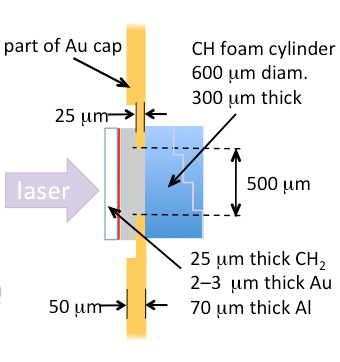
\includegraphics[width=0.25\textwidth]{../figs_NTH/WDFEOS/Target_scheme.png} 
&
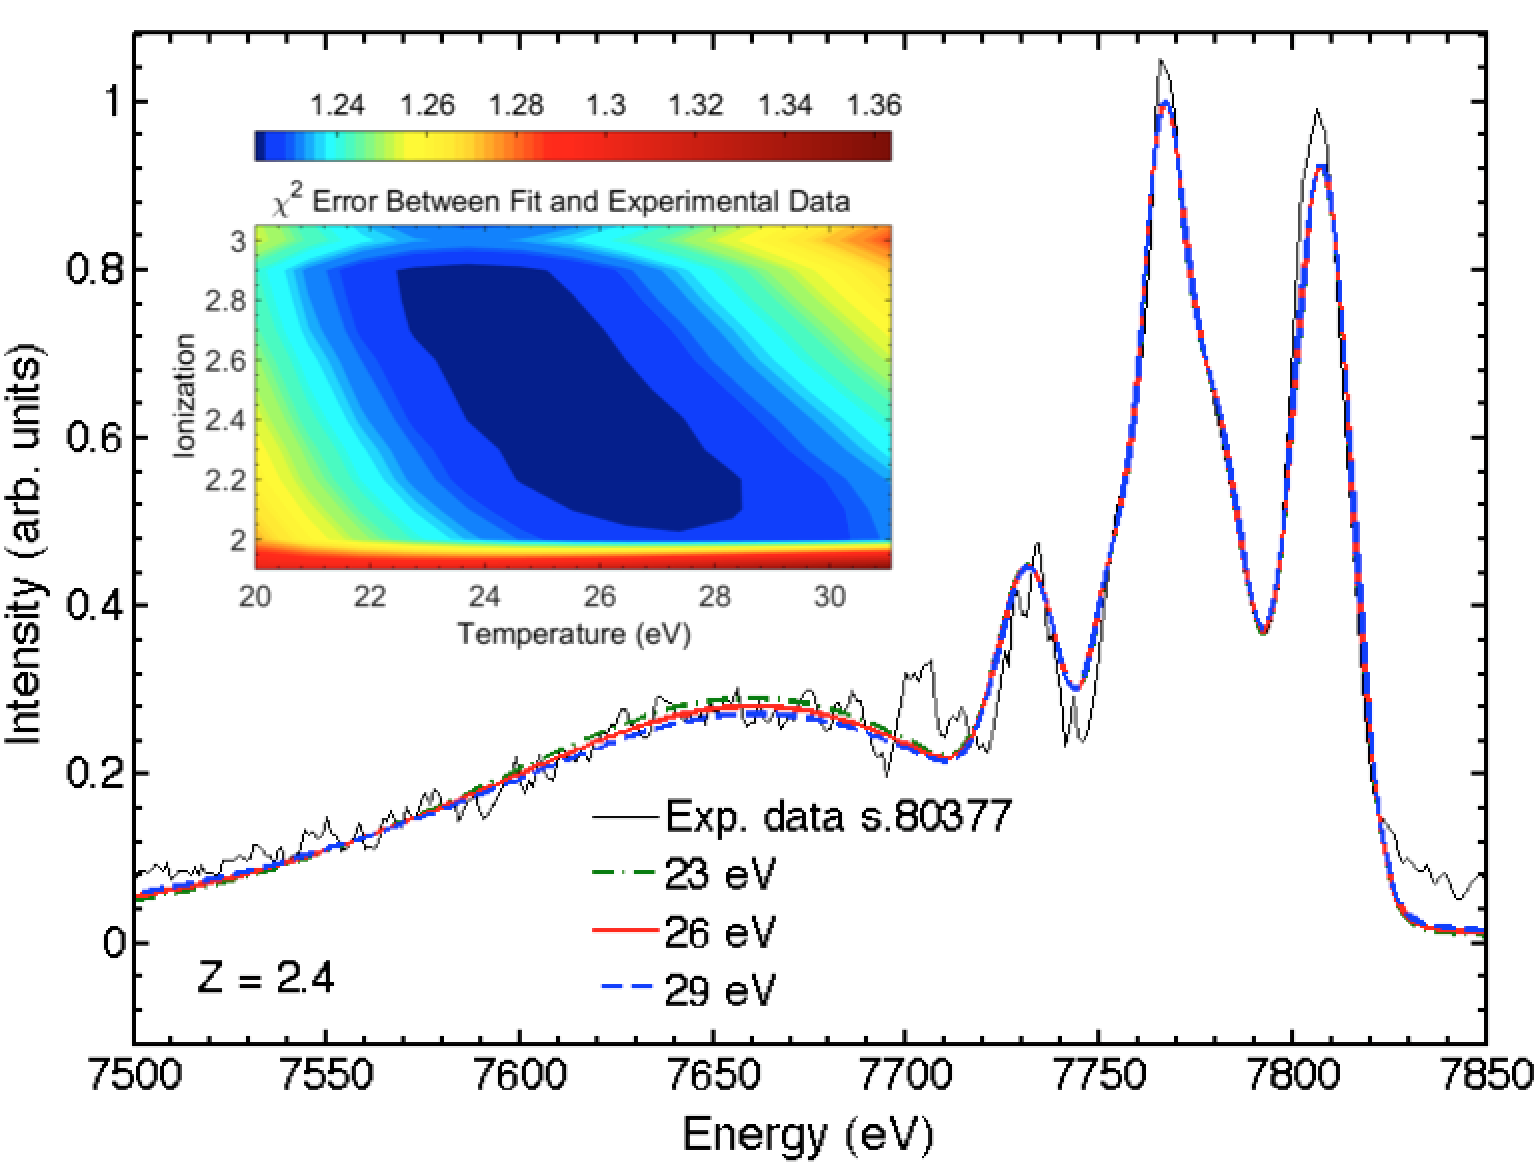
\includegraphics[width=0.32\textwidth]{../figs_NTH/WDFEOS/XRTS_CH_fit.png}
\\
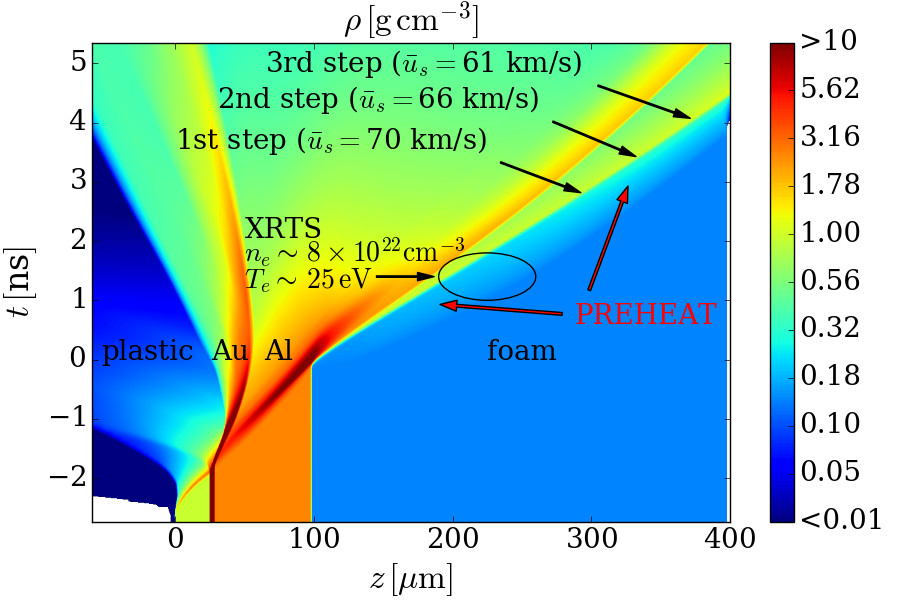
\includegraphics[width=0.36\textwidth]{../figs_NTH/WDFEOS/fig3.png} 
&
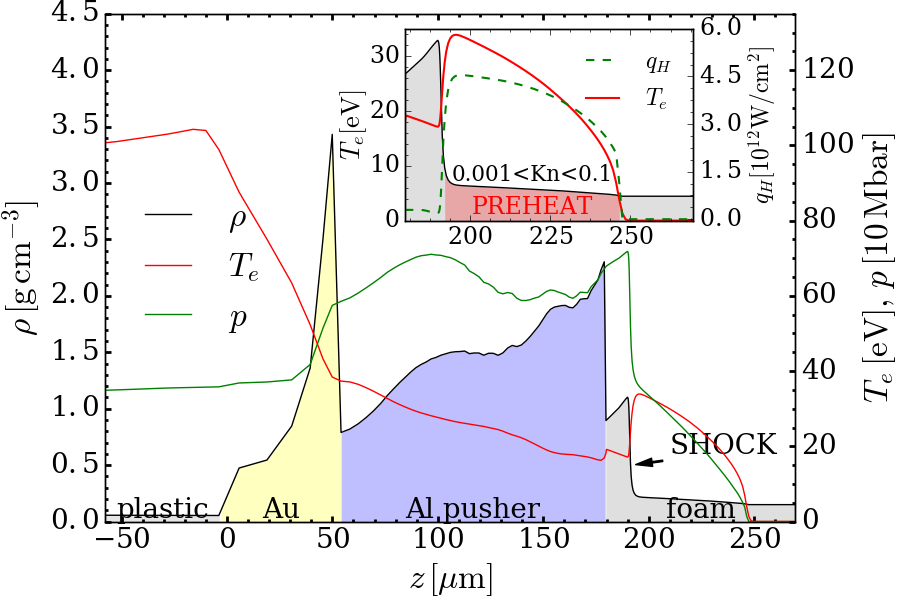
\includegraphics[width=0.36\textwidth]{../figs_NTH/WDFEOS/fig4.png} 
\end{tabular}
%\caption{.}
\label{WDFEOS_fig}
\end{center}
\end{figure}
flat 2 ns laser pulse, 8$\times$10$^{14}$ Wcm2, 
300 $\mu$m thick foam ($\rho=0.13$ g/cm$^3$) 
\end{center}
\end{frame}

\begin{frame}
\begin{center}
\begin{figure}
\begin{center}
\begin{tabular}{c}
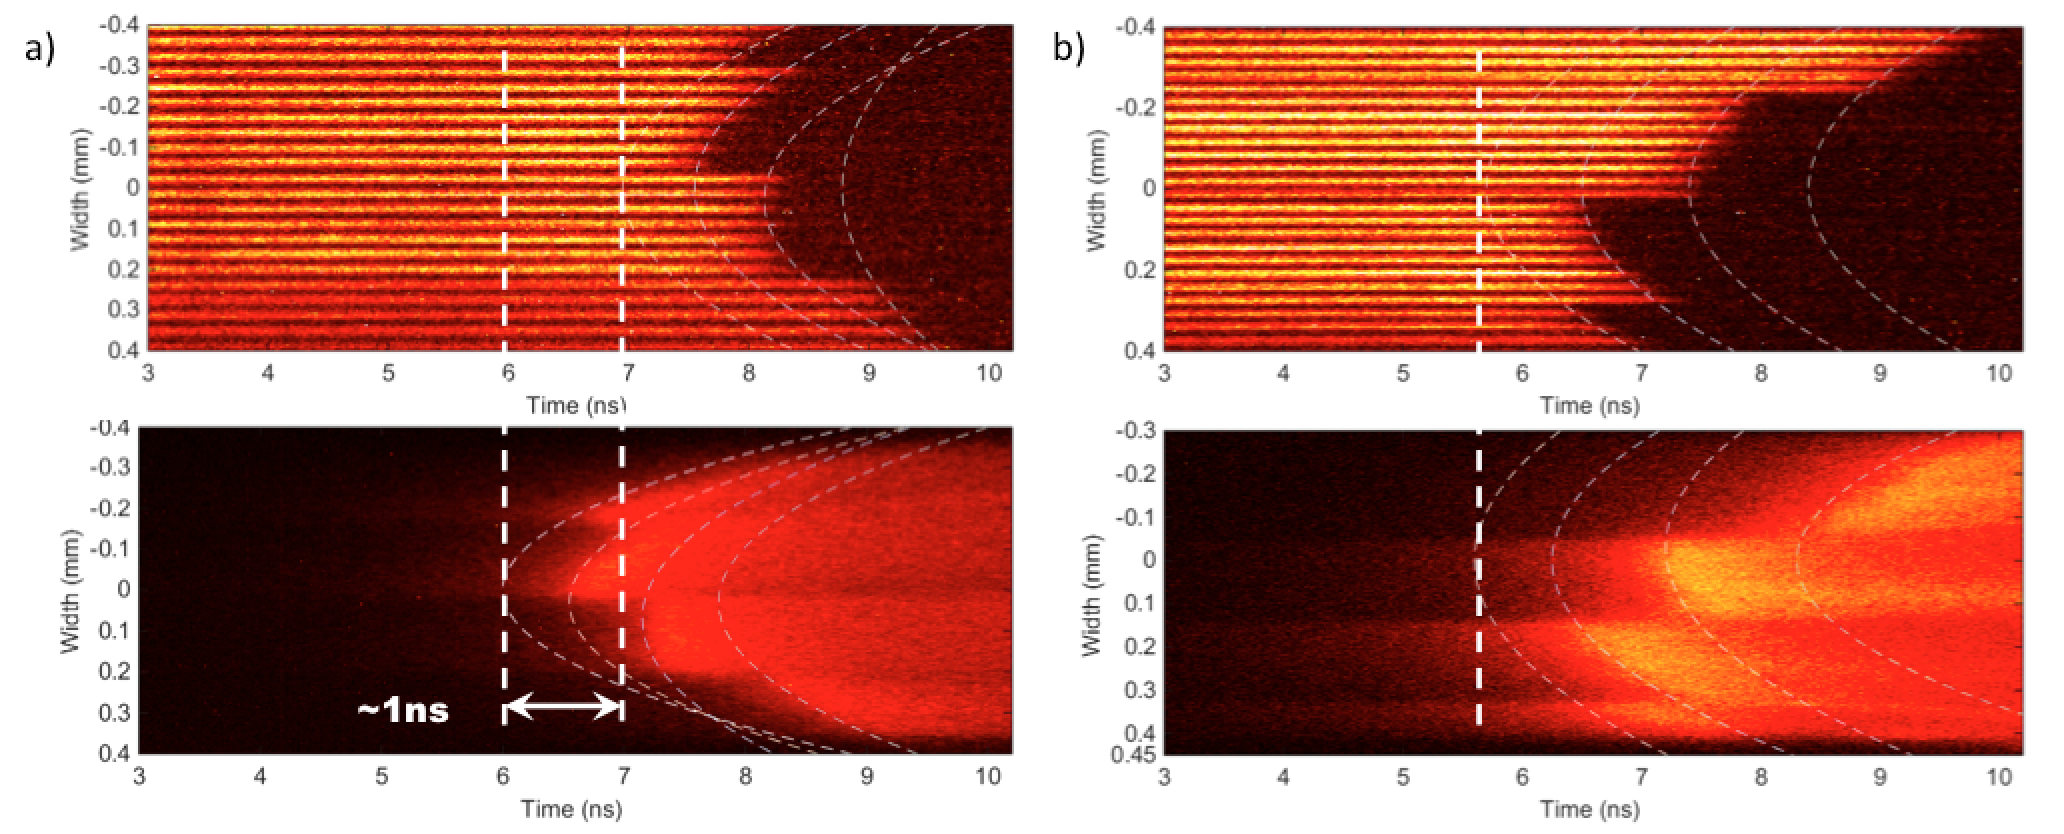
\includegraphics[width=1.0\textwidth]{../figs_NTH/WDFEOS/Visar_SOP_complete.png} 
\end{tabular}
%\footnote{SOP, VISAR, and XRTS combined diagnostics introduced by 
%K. Falk et al. PoP 2014.}
%\caption{.}
\label{WDFEOS_fig}
\end{center}
\end{figure}
a) recent experiment with new phase-plates, b) previous experiment
\end{center}
\end{frame}

\begin{frame}
\begin{center}
{\large Rankine-Hugoniot jump condition analysis}
\begin{figure}
\begin{center}
\begin{tabular}{ll}
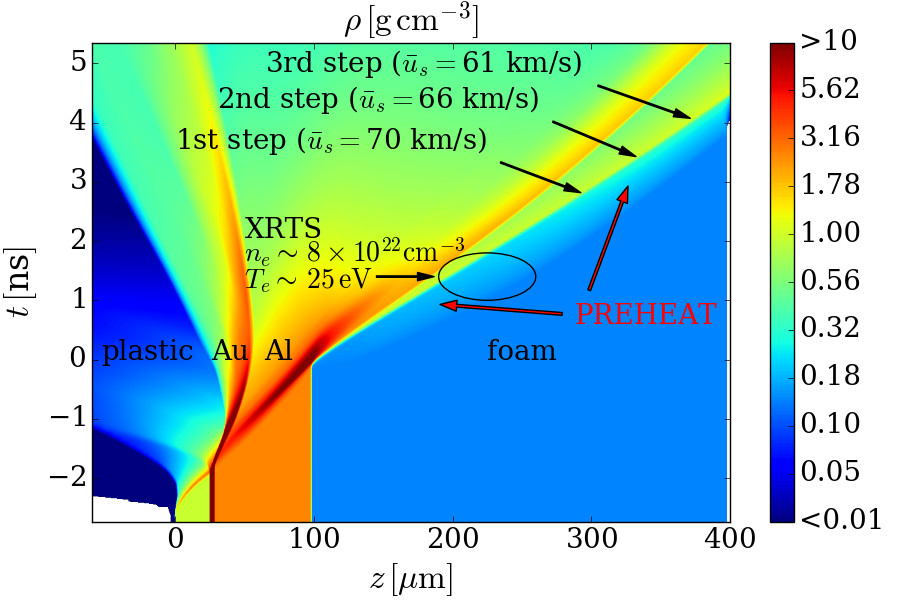
\includegraphics[width=0.36\textwidth]{../figs_NTH/WDFEOS/fig3.png} 
&
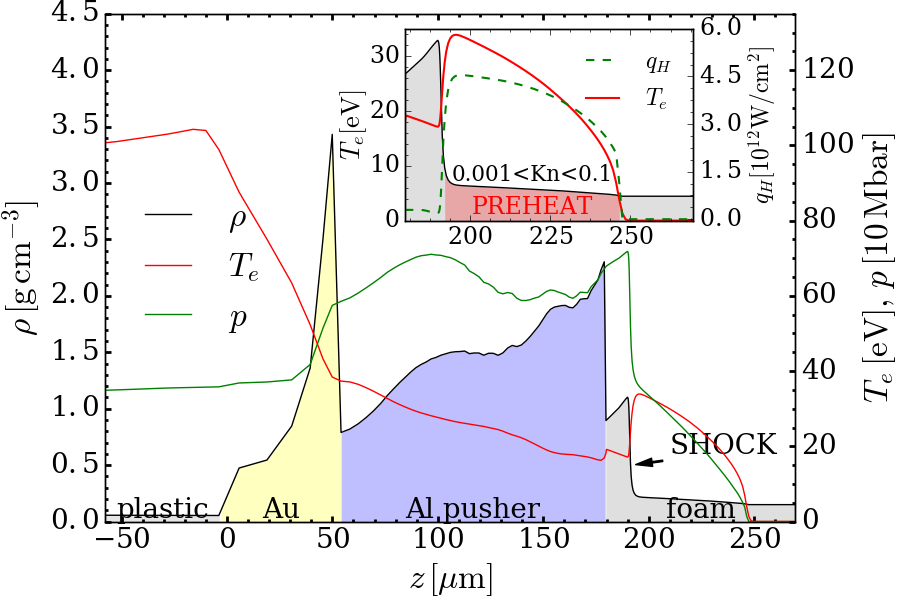
\includegraphics[width=0.34\textwidth]{../figs_NTH/WDFEOS/fig4.png} 
\end{tabular}
%\caption{.}
\label{RH_fig}
\end{center}
\end{figure}
\begin{eqnarray}
u_s (\rho_0 - \rho_1) &=& \rho_0 u_0 - \rho_1 u_1 
\nonumber\\
u_s (\rho_0 u_0 - \rho_1 u_1) &=& (\rho_0 u_0^2 + p_0) - (\rho_1 u_1^2 + p_1)
\nonumber \\
u_s (E_0 - E_1) &=& u_0 (E_0 + p_0) - u_1 (E_1 + p_1) + 
\colorimportant{({q_e}_0+{q_R}_0) - ({q_e}_1+{q_R}_1)}
\nonumber
\end{eqnarray}
%Rankine-Hugoniot jump condition due to the mass conservation
%given by 
%
%($\rho_1 = 0.81$ g/cm$^3$, $v_1 = 6.72\times10^{-6}$ cm/s) and 
%($\rho_0 = 0.2$ g/cm$^3$, $v_0 = 2.9\times10^{-6}$ cm/s) 
%
%suggests the shock 
%velocity \colorimportant{80 km/s} 
%(an excellent agreement with our simulations). 
\begin{block}{Rankine-Hugoniot jump condition of energy}
\begin{equation}
 u_s = \frac{\Delta q_{tot}}{\Delta E} = 
 \frac{u_0 (E_0 + p_0) - u_1 (E_1 + p_1) + 
\colorimportant{({q_e}_0+{q_R}_0) - ({q_e}_1+{q_R}_1)}}{E_0 - E_1} \nonumber
\end{equation}
\end{block}

%The~classical Hugoniot theory (neglecting the~electron 
%energy flux) leads to a~much lower shock velocity $\approx$ \colorf{60 km/s}.
The high shock velocity \colorimportant{70 km/s} is because 
the~electron flux contribution 
$\colorimportant{{q_e}_1 - {q_e}_0 \approx -2(p_1 u_1 - p_0 u_0)\approx 
0.16(u_1(E_1 + p_1) - u_0(E_0 + p_0))}$, 

which is comparable to the~hydrodynamics flux contribution.
\end{center}
\end{frame}

\begin{frame}
\begin{center}
{\large Nonlocal vs. SH diffusion}
\begin{figure}
\begin{center}
\begin{tabular}{ll}
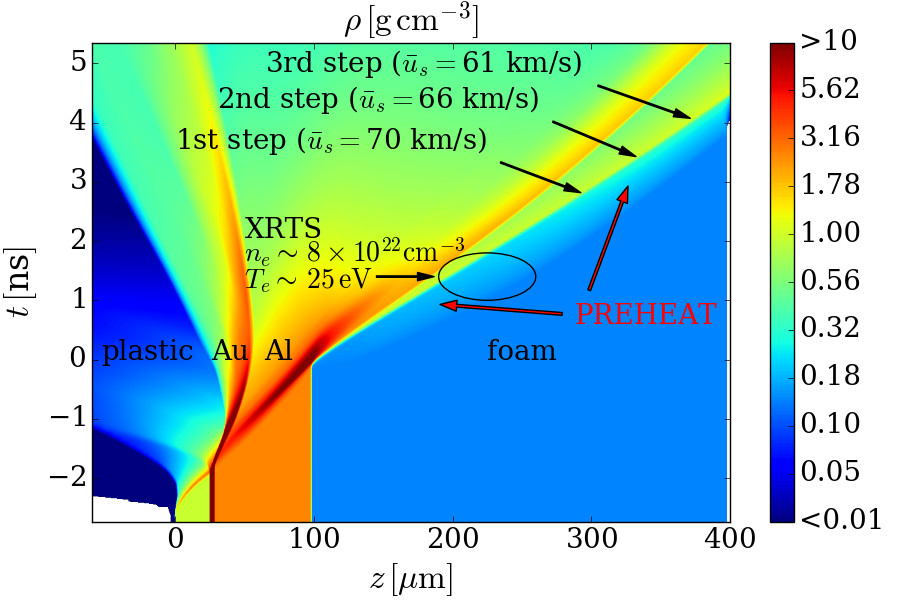
\includegraphics[width=0.36\textwidth]{../figs_NTH/WDFEOS/fig3.png} 
&
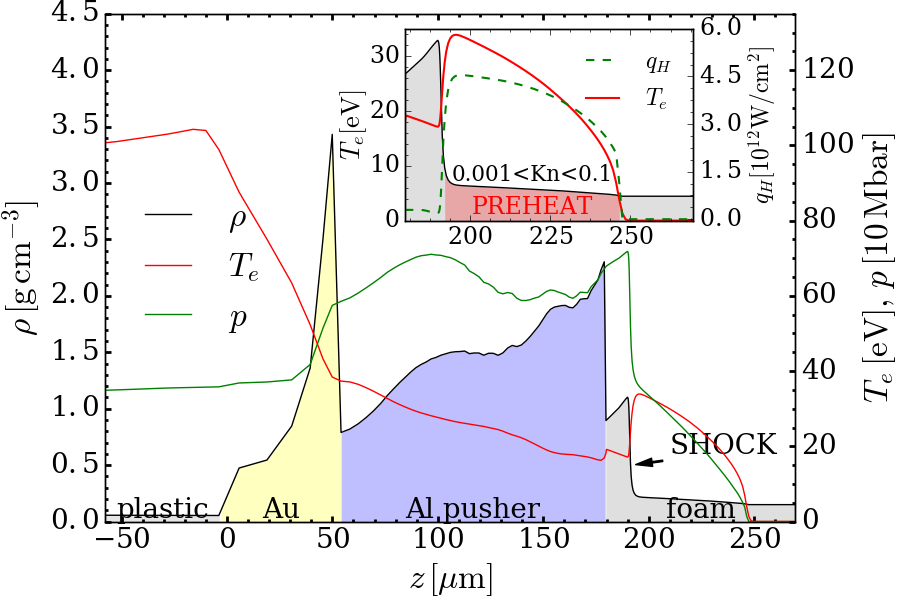
\includegraphics[width=0.34\textwidth]{../figs_NTH/WDFEOS/fig4.png} 
\\
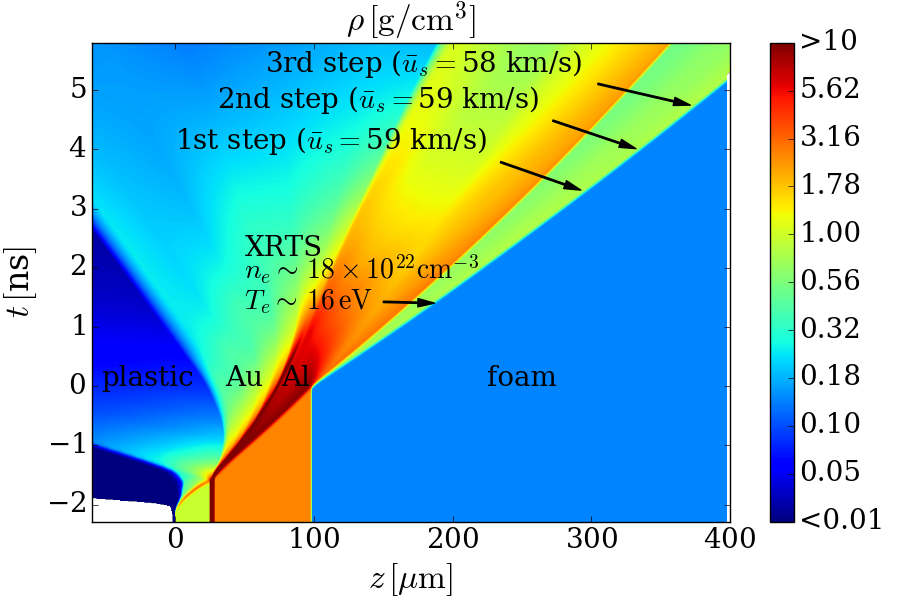
\includegraphics[width=0.36\textwidth]{../figs_NTH/WDFEOS/fig5.png} 
&
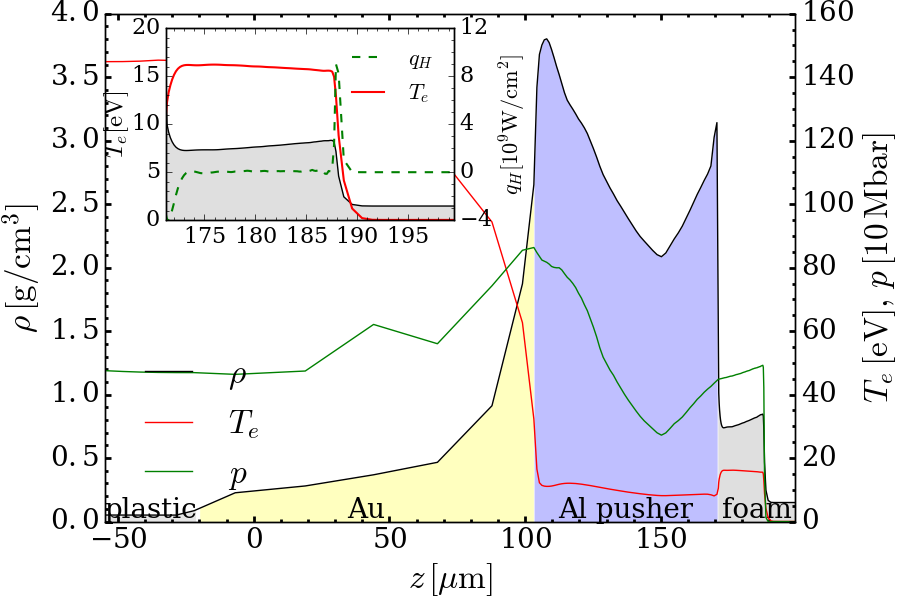
\includegraphics[width=0.34\textwidth]{../figs_NTH/WDFEOS/fig6.png} 
\end{tabular}
%\caption{.}
\label{RH_fig}
\end{center}
\end{figure}
Effective mean free path was 4.1$\times v_T$, according to LANL code ATOMIC 
the mean free path in WDM foam increases $\approx$ 30$\%$.
\end{center}
\end{frame}

%\begin{comment} % LANL
\begin{frame}
\begin{center}
{\large X-ray preheat analysis}
\begin{figure}
\begin{center}
\begin{tabular}{ll}
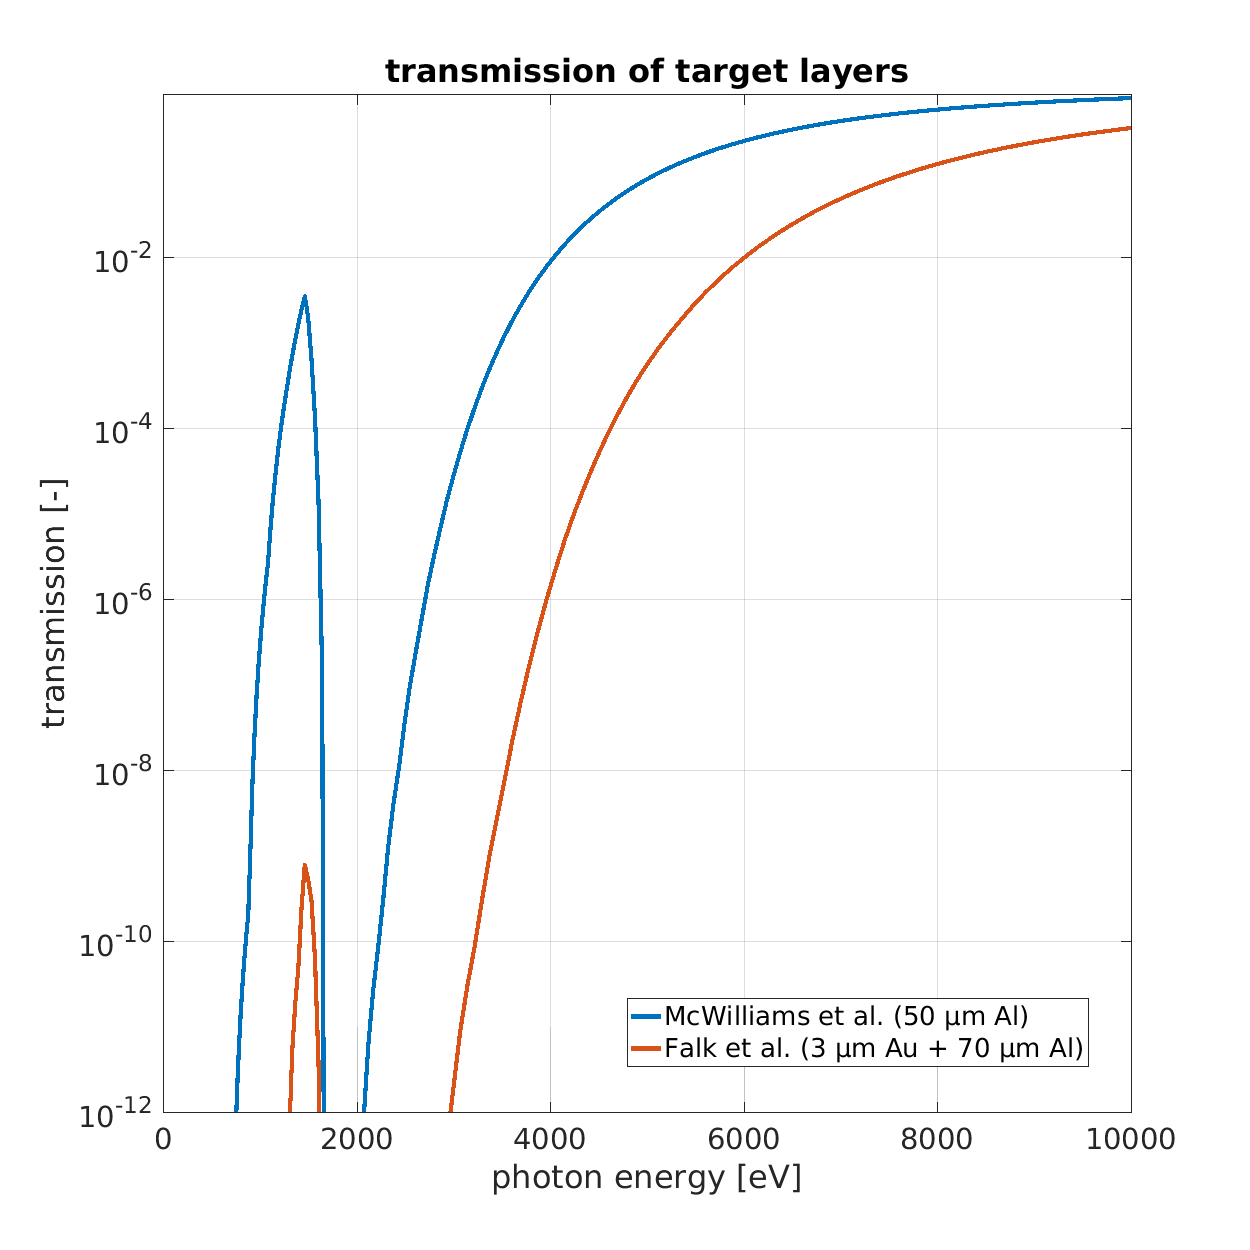
\includegraphics[width=0.36\textwidth]{../figs_NTH/WDFEOS/Transmission.png} 
&
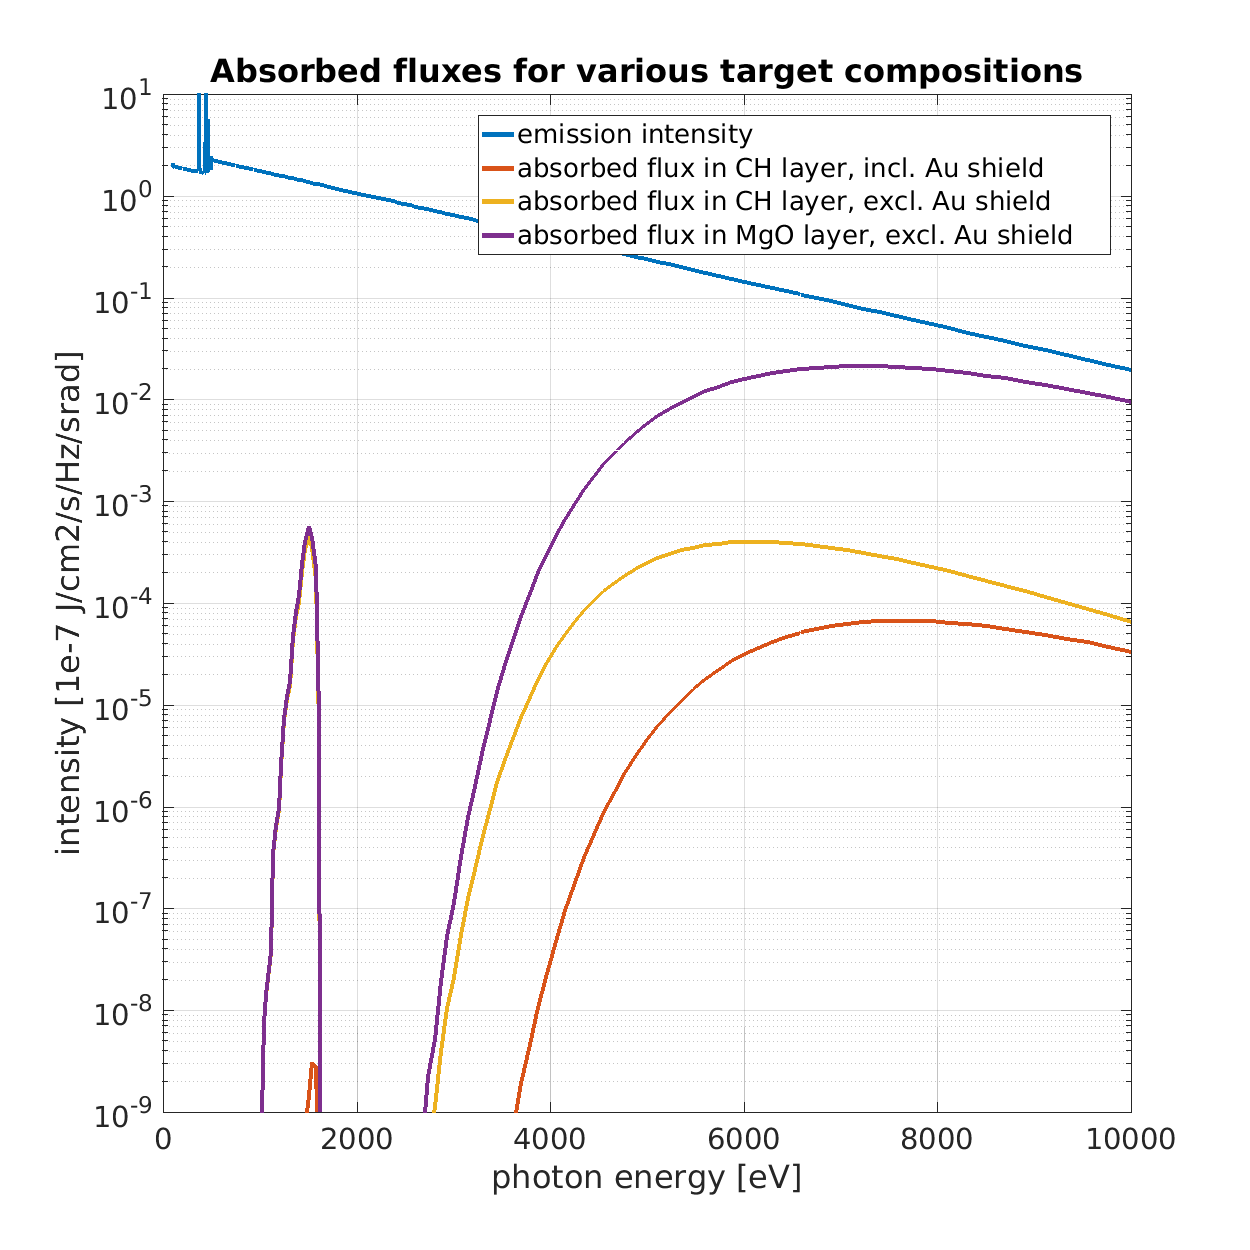
\includegraphics[width=0.36\textwidth]{../figs_NTH/WDFEOS/Absorbed_flux.png} 
\end{tabular}
%\caption{.}
\label{RH_fig}
\end{center}
\end{figure}
Significant part of x-rays $<$ 2keV (penetration depth is small) $\rightarrow$ 
energy absrobed in the surface of the foam is $\approx$ 670 J/cm3. 
Absorbed energy density by nonlocal electrons $\approx$ 2.7e6 J/cm3.
\end{center}
\end{frame}
%\end{comment} % LANL

\begin{frame}
%\myheading{\colorimportant{P}lasma \colorimportant{E}uler and 
%\colorimportant{T}ransport \colorimportant{E}quations
%nonlocal hydro code}
\myheading{Conclusions}
\begin{block}{Plasma Euler and Transport Equations
hydro code \colorimportant{PETE}}
\begin{tabular}{c|c}
\begin{pcolumn}{0.5}
\begin{eqnarray}
  \frac{\partial \rho}{\partial t} &=& -\nabla\cdot(\rho\vect{u})\, , 
  \nonumber
  \\
  \frac{\partial \rho \vect{u}}{\partial t} &=& -\nabla\cdot(\rho\vect{u}
  \otimes\vect{u} + p\, \matr{I})\, ,
  \nonumber
  \\ 
  \frac{\partial E}{\partial t} &=& -\nabla\cdot(E \vect{u} + p\vect{u} +
  \vect{q}_L + \colorimportant{\vect{q}_e + \vect{q}_R})\, ,
  \nonumber
\end{eqnarray} 
density $\rho$, fluid velocity $\vect{u}$, total energy 
$E(T)$, pressure $p(\rho, T)$, 
laser energy flux $\vect{q}_L$, 
electron heat flux $\vect{q}_e$, radiation flux $\vect{q}_R$.
\end{pcolumn} &
\begin{pcolumn}{0.4}
\begin{eqnarray}
  %\frac{1}{c}\frac{\partial I^{\, p}}{\partial t} + 
  \vect{n}\cdot\nabla I^{\, p} &=& 
  \frac{\sigma^{p} T_e - I^{\, p}}{\lambda^{p}}\, , 
  \nonumber
  \\
  \vect{q}_R &=& \int_{4\pi}\vect{n}\, I^{\, p}\, \dI\vect{n}\,  ,
  \nonumber
  \\
  \hline\nonumber\\
  %\frac{1}{\bar{v}}\frac{\partial I^e}{\partial t} +
  \vect{n}\cdot\nabla I^e 
  &=& 
  \frac{\sigma^e T_e - I^e}{\lambda^e}\, , 
  \nonumber
  \\
  \vect{q}_e &=& \int_{4\pi}\vect{n}\, I^e\, \dI\vect{n}\,  ,
  \nonumber
\end{eqnarray}

\end{pcolumn}
\end{tabular}
\end{block}

\begin{itemize}
\item Lagrangian frame, 2T single fluid, IB laser deposition, SESAME
%\item SESAME/QEOS/FEOS/BADGER equation of state
%\item Inverse-bremsstrahlung laser deposition (Stationary Maxwell Equation),
%intensities between 10$^{11}$ -- 10$^{15}$ W/cm$^2$
\item Nonlocal radiation and electron transport
\item Inherent coupling of nonlocal transport and energy equations via 
$I = a(\vect{x}, \vect{n})\, T_e + b(\vect{x}, \vect{n})$, 
which leads to a temperature dependence of energy fluxes 
$\colorimportant{\vect{q}_e + \vect{q}_R = \matr{A}\, T_e + \vect{b}}$
\item Extension of PETE to 2D Cartesian/axisymmetric based on HONTS and Laghos 
soon 
\end{itemize}
\begin{figure}
\begin{center}
\begin{tabular}{ccc} 
  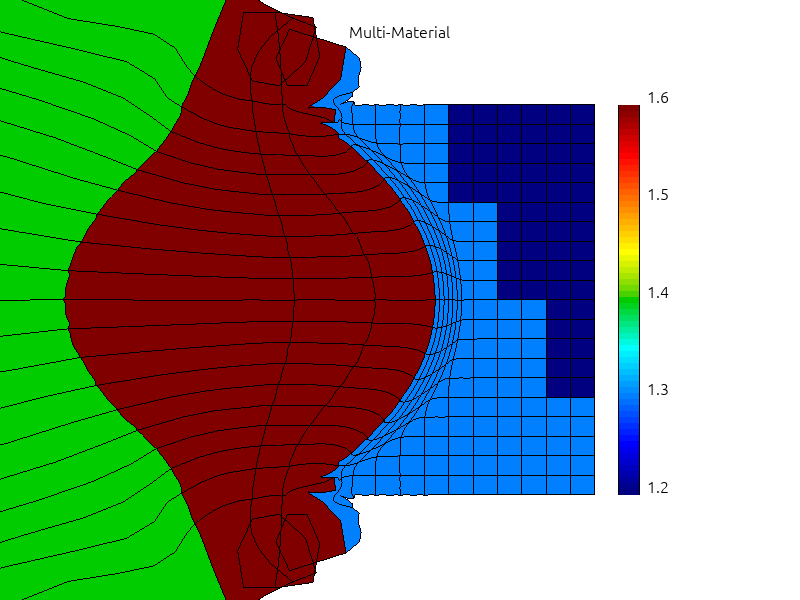
\includegraphics[width=0.25\textwidth]{../figs_NTH/results/OmegaLaser/material_77.png}
  &
  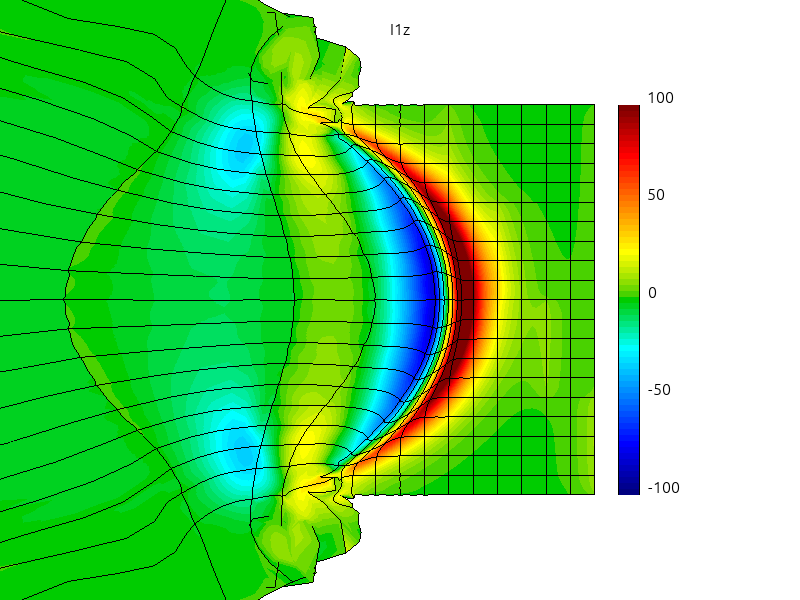
\includegraphics[width=0.25\textwidth]{../figs_NTH/results/OmegaLaser/nonlocalI1z_77.png}
  &
  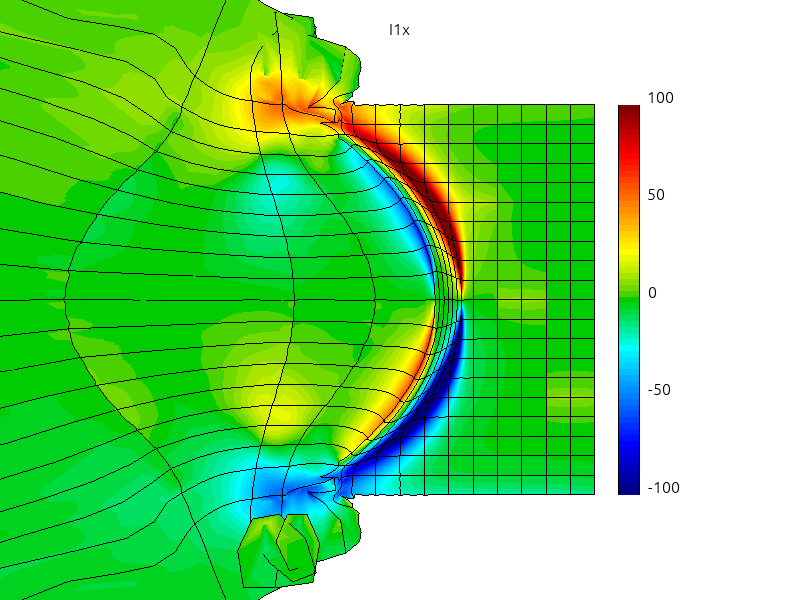
\includegraphics[width=0.25\textwidth]{../figs_NTH/results/OmegaLaser/nonlocalI1x_77.png}
\end{tabular}
\end{center}
\end{figure}
%Based on \colorimportant{MFEM}, a free, lightweight, scalable C++ library for 
%finite element methods developed at Lawrence Livermore National Laboratory, CA.
%\colorimportant{"My finite element library is higher order than yours..."}
\end{frame}

%\end{comment} % Extensive NTH model
\newcommand{\fzero}{f_0}
\newcommand{\fone}{\boldsymbol{f}_1}
\newcommand{\ftwo}{\boldsymbol{f}_2}
\newcommand{\pv}{\frac{\partial}{\partial v}}
\newcommand{\nuee}{\nu_{ee}}
\newcommand{\nut}{\nu_{tot}}
\newcommand{\fM}{f_M}
\begin{frame}
\begin{center}
{\large Nonlocal Transport Magneto-Hydrodynamics (NTMHD) model}  
\begin{equation}
  %\frac{1}{|\vect{v}|}\frac{\partial f}{\partial t} + 
  \vect{n}\cdot\nabla_x f + \frac{q_e}{m_e |\vect{v}|}\left(\vect{E}\cdot
  \vect{n}\frac{\partial}{\partial |\vect{v}|}f 
  + \left(\frac{\vect{E}}{|\vect{v}|}+\frac{\vect{n}}{c}\times\vect{B}\right)\cdot\nabla_{\vect{n}} f\right)
  = 
  \frac{f_{MB}(|\vect{v}|, T_e) - f}{\lambda_{ei}(|\vect{v}|^4)} 
  %+ \frac{|\vect{v}|}{\lambda_{ee}}\frac{\partial}{\partial |\vect{v}|}
  %\left(\frac{v_T^2}{|\vect{v}|}\frac{\partial}{\partial |\vect{v}|} + 1\right) 
  %\left(f - f_0\right) 
  \nonumber
\end{equation}
\begin{block}{NTH Electric field vs. generalized Ohm's law}
\begin{eqnarray}
   \sum_g \int_{\Delta v^g} \frac{e}{m_e v}\left(\frac{1}{v}\pv 
   \left( v^2 \ftwo\right) + \left(\ftwo - \fzero\matr{I}\right)\right) \dI v
   \cdot\vect{E} &=& 
   \sum_g \int_{\Delta v^g} v\nabla\cdot\ftwo 
   + (\nuee + \nut) \fone \dI v
   + \sum_g \int_{\Delta v^g} \frac{e}{m_e c} \fone\dI v \times\vect{B}
   \nonumber \\
   %\vect{E} + \frac{v_i}{c}\times\vect{B} &=&  
   \vect{E} &=&  
   \frac{1}{e n_e}\left(\vect{R}_T -\nabla p_e\right) + 
   \frac{\vect{j}}{e n_e \sigma} + \frac{1}{e n_e c}\vect{j}\times\vect{B}
   \nonumber
\end{eqnarray}
\end{block}
\begin{eqnarray}
  \nabla\times\vect{E} &=& -\frac{1}{c}\frac{\partial \vect{B}}{\partial t}
  \quad\qquad (\text{life of magnetic field} \vect{B}) 
  \nonumber \\
  \nabla\times\vect{B} &=& \frac{4\pi}{c}
  \left(\vect{j} + \tilde{\vect{j}}\right)\quad (\text{quasi-neutrality} 
  \nabla\cdot\left(\vect{j} + \tilde{\vect{j}}\right) = 0) 
  \nonumber
\end{eqnarray}
Applying generalized Ohm's and Ampere's laws, we get
\begin{equation}
  %\nabla\times\tilde{\vect{E}} = 
   \nabla\times\vect{E} = 
  \nabla\times\left(
  \frac{1}{e n_e}\left(\vect{R}_T -\nabla p_e\right) + 
  \frac{c}{e n_e \sigma 4\pi}\nabla\times\vect{B} 
  - \frac{\tilde{\vect{j}}}{e n_e \sigma} + 
  \frac{1}{e n_e c}\vect{j}\times\vect{B}\right)
  \nonumber
\end{equation}
\begin{block}{Maxwell Equations for Hydrodynamics - dynamo equation for 
nonlocal magnetic field source}
\begin{equation}
  \frac{1}{c}\frac{\partial \vect{B}}{\partial t} = 
  - \nabla\times\frac{1}{e n_e c}\vect{j}\times\vect{B}
  - \nabla\times\frac{c}{e n_e \sigma 4\pi}\nabla\times\vect{B}
  - \nabla\times \left(
  \frac{\sum_g \int_{\Delta v^g} v\nabla\cdot\ftwo \dI v}
  {\sum_g \int_{\Delta v^g} \frac{e}{m_e v}\left(\frac{1}{v}\pv 
  \left( v^2 \ftwo\right) + \left(\ftwo - \fzero\matr{I}\right)\right) \dI v} + 
  - \frac{\tilde{\vect{j}}}{e n_e \sigma}\right)
  \nonumber
\end{equation}
\end{block}
\footnote{Kingham and Bell PRL 2002}
\end{center}
\end{frame}



\begin{frame}
\begin{center}
{\large Vlasov-Fokker-Planck simulations}
\begin{figure}
\begin{center}
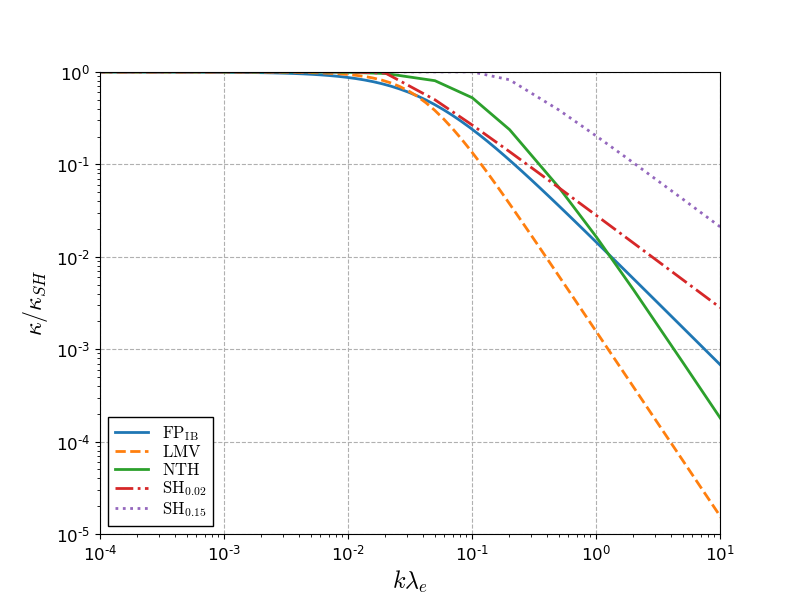
\includegraphics[width=0.7\textwidth]{../figs_NTH/VFP_Epperlein.png} 
%\caption{.}
\label{RH_fig}
\end{center}
\end{figure}
\footnote{Kinetic simulations provided by Jan Nikl (ELI Beamlines).}
%\begin{itemize}
%  \item show NTH
%  \item point out heat flux limiter
%\end{itemize}
\end{center}
\end{frame}

\begin{comment} % Efield
\begin{frame}
\begin{center}
{\large Electric Field}

The M1 model reads
\begin{eqnarray}
   v\nabla\cdot\fone - \frac{e}{m_e v}\frac{1}{v}\pv \left( v^2 \fone\right)
   \cdot\vect{E} &=& \nuee v \pv(\fzero - \fM)\nonumber\\
   v\nabla\cdot\ftwo - \frac{e}{m_e v}\left(\frac{1}{v}\pv 
   \left( v^2 \ftwo\right) + \left(\ftwo - \fzero\matr{I}\right)\right)
   \cdot\vect{E}  &=& \nuee v \pv \fone - \nut \fone\nonumber
\end{eqnarray}
From nonlocal momentum equation, we can evaluate the electric field
\begin{equation}
   \sum_g \int_{\Delta v^g} - \frac{e}{m_e v}\left(\frac{1}{v}\pv 
   \left( v^2 \ftwo\right) + \left(\ftwo - \fzero\matr{I}\right)\right) \dI v
   \cdot\vect{E} = 
   \sum_g \int_{\Delta v^g} - v\nabla\cdot\ftwo 
   + \nuee \pv \left( v \fone \right) 
   - (\nuee + \nut) \fone \dI v
   \nonumber
\end{equation}
 
\begin{block}{Quasi-neutrality}
\begin{equation}
   \sum_g \int_{\Delta v^g} - \frac{e}{m_e v (\nuee + \nut)}\left(\frac{1}{v}\pv 
   \left( v^2 \ftwo\right) + \left(\ftwo - \fzero\matr{I}\right)\right) \dI v
   \cdot\vect{E} = 
   \sum_g \int_{\Delta v^g} - \frac{v}{(\nuee + \nut)}\nabla\cdot\ftwo \dI v
   \nonumber
\end{equation}
\end{block}
which is a M1 nonlocal definition of the electric field similar to
\footnote{Shkarofsky PRL 1979, Kingham and Bell PRL 2002}
\begin{equation}
  \vect{E} = \frac{m_e}{e 6 n_e}\frac{\nabla n_e <v^5>}{<v^3>}
  \nonumber
\end{equation}
\end{center}
\end{frame}
\end{comment} % Efield

\begin{frame}
\begin{center}
%{\large Nonlocal vs. diffusive transport model}
\begin{figure}
\begin{center}
\begin{tabular}{cc}
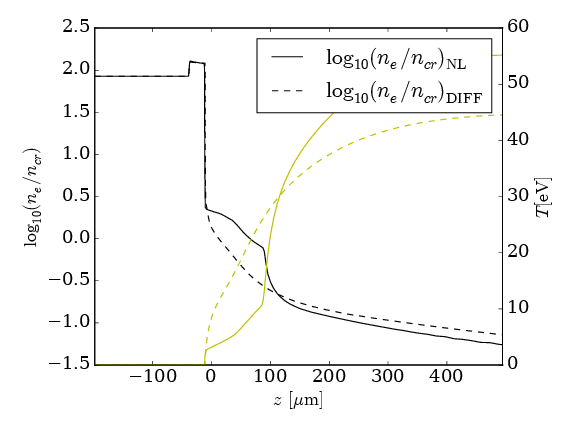
\includegraphics[width=0.315\textwidth]{../figs_NTH/Prepulse/CH_1e22_nencs_Tes.png} 
&
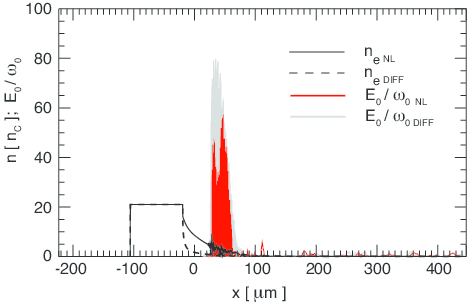
\includegraphics[width=0.35\textwidth]{../figs_NTH/Prepulse/PIC_t_7000.png}
\end{tabular}
%\caption{.}
\label{L4_fig}
\end{center}
\end{figure}

\begin{figure}
\begin{center}
\begin{tabular}{c}
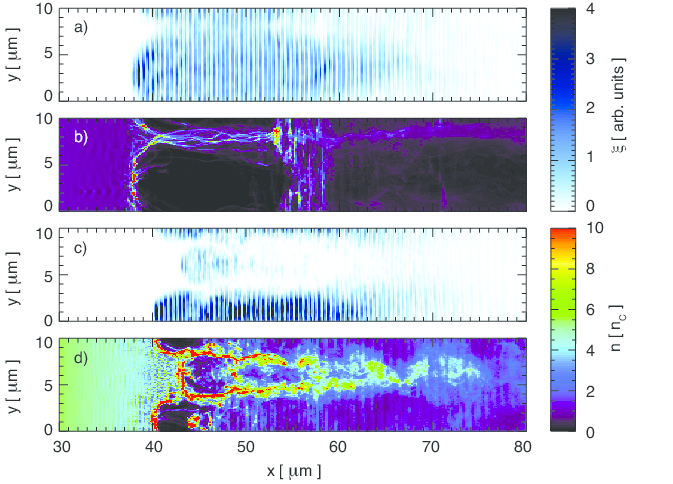
\includegraphics[width=0.45\textwidth]{../figs_NTH/Prepulse/PIC_2D.png}
\footnote{OSIRIS PIC simulations by Marija Vranic 2017.}
\end{tabular}
%\caption{.}
\label{L4_PIC_fig}
\end{center}
\end{figure}
\end{center}
\end{frame}

\begin{comment} % M1comment
\begin{frame}
\begin{center}
{\large Hyperbolic M1 Model}
\begin{eqnarray}
   v\nabla\cdot\fone - \frac{e}{m_e v}\frac{1}{v}\pv \left( v^2 \fone\right)
   \cdot\vect{E} &=& \nuee v \pv(\fzero - \fM)\nonumber\\
   v\nabla\cdot\ftwo - \frac{e}{m_e v}\left(\frac{1}{v}\pv 
   \left( v^2 \ftwo\right) + \left(\ftwo - \fzero\matr{I}\right)\right)
   \cdot\vect{E}  &=& \nuee v \pv \fone - \nut \fone\nonumber
\end{eqnarray}
where the system of unknowns in Cartesian coordinates
\begin{equation}
\fzero\, ,\quad \fone = [f_{1 x}, f_{1_y}]\, ,\quad \ftwo = 
  \begin{bmatrix}
    {\ftwo}_{xx} & {\ftwo}_{xy} \\
	{\ftwo}_{yx} & {\ftwo}_{yy} 
  \end{bmatrix}
  = \matr{X}\, \fzero
  \nonumber
\end{equation}
can be represented as a vector field hyperbolic problem
\begin{equation}
  - \nuee \pv \vect{u} + \nabla\cdot\matr{F} = \frac{e}{m_e v}\frac{1}{v}
  \pv\matr{F}\cdot\vect{E} - \vect{S}
  \nonumber
\end{equation} 
\begin{equation}
   \vect{u} =
   \begin{bmatrix}
    \fzero \\
	{\fone}_x \\
	{\fone}_y 
  \end{bmatrix}
  \, ,\quad 
  \matr{F} = 
  \begin{bmatrix}
    {\fone}_x & {\fone}_y \\
	{\ftwo}_{xx} & {\ftwo}_{xy} \\
	{\ftwo}_{yx} & {\ftwo}_{yy} 
  \end{bmatrix}
  \, ,\quad
  \vect{S} =
  \begin{bmatrix}
    \nuee v \pv\fM \\
	\nut{\fone}_x + [{\ftwo}_{xx} - \fzero, {\ftwo}_{xy}]\cdot\vect{E} \\
	\nut{\fone}_y + [{\ftwo}_{yx}, {\ftwo}_{yy} - \fzero]\cdot\vect{E}
  \end{bmatrix} 
  \nonumber
\end{equation}
\end{center}
\end{frame}

\begin{frame}
\begin{center}
{\large Numerical Scheme}

Transport equation
\begin{equation}
  - \nuee \pv \vect{u} + \nabla\cdot\matr{F} = \frac{e}{m_e v}\frac{1}{v}
  \pv\matr{F}\cdot\vect{E} - \vect{S}
  \nonumber
\end{equation} 
is discretized in space and velocity using discrete divergence analog 
$\matr{D}$ and forward Euler finite differences in velocity as 
\begin{equation}
  \nuee \frac{\vect{u}^{g+1} - \vect{u}^{g}}{\Delta v} = 
  \matr{D}\cdot\matr{F}^{g+1} - \frac{e}{m_e v}\frac{1}{v}
  \frac{\matr{F}^{g+1} - \matr{F}^{g}}{\Delta v}\cdot\vect{E} + \vect{S}^{g}
  + \Gamma(\vect{u}^{g+1}, \matr{F}^{g+1})
  \nonumber
\end{equation} 
Such a scheme can be easily inverted (element-wise) to obtain $\fzero$ and
$\fone$
\begin{block}{Discrete version of M1}
\begin{equation}
\matr{A}\cdot\vect{u}^{g} = \nuee \vect{u}^{g+1} - \matr{D}\cdot\matr{F}^{g+1} 
  + \frac{e}{m_e v}\frac{1}{v}\matr{F}^{g+1}\cdot\vect{E} 
  + \Delta v \Gamma(\vect{u}^{g+1}, \matr{F}^{g+1})
  - \vect{S}(n_e^{g}, T^{g})  
  \nonumber
\end{equation}
where the coupling to hydrodynamics goes via $n_e$ and $T$ in the source $S$.
\end{block}

\begin{equation}
  \matr{F}_{LF} = 
  0.5\left(\matr{F}^{+} + \matr{F}^{-}\right)\cdot\vect{n}_{\Gamma} + 
  0.5\lambda\left(\vect{u}^{+} - \vect{u}^{-} \right)
  \, ,\quad
  \Delta v \le \frac{S_t}{h^{-1}}
  \nonumber
\end{equation}

\end{center}
\end{frame}

\begin{frame}
\begin{center}
{\large Electric Field}

The M1 model reads
\begin{eqnarray}
   v\nabla\cdot\fone - \frac{e}{m_e v}\frac{1}{v}\pv \left( v^2 \fone\right)
   \cdot\vect{E} &=& \nuee v \pv(\fzero - \fM)\nonumber\\
   v\nabla\cdot\ftwo - \frac{e}{m_e v}\left(\frac{1}{v}\pv 
   \left( v^2 \ftwo\right) + \left(\ftwo - \fzero\matr{I}\right)\right)
   \cdot\vect{E}  &=& \nuee v \pv \fone - \nut \fone\nonumber
\end{eqnarray}
From nonlocal momentum equation, we can evaluate the electric field
\begin{equation}
   \sum_g \int_{\Delta v^g} - \frac{e}{m_e v}\left(\frac{1}{v}\pv 
   \left( v^2 \ftwo\right) + \left(\ftwo - \fzero\matr{I}\right)\right) \dI v
   \cdot\vect{E} = 
   \sum_g \int_{\Delta v^g} - v\nabla\cdot\ftwo 
   + \nuee \pv \left( v \fone \right) 
   - (\nuee + \nut) \fone \dI v
   \nonumber
\end{equation}
 
\begin{block}{Quasi-neutrality}
\begin{equation}
   \sum_g \int_{\Delta v^g} - \frac{e}{m_e v (\nuee + \nut)}\left(\frac{1}{v}\pv 
   \left( v^2 \ftwo\right) + \left(\ftwo - \fzero\matr{I}\right)\right) \dI v
   \cdot\vect{E} = 
   \sum_g \int_{\Delta v^g} - \frac{v}{(\nuee + \nut)}\nabla\cdot\ftwo \dI v
   \nonumber
\end{equation}
\end{block}
which is a M1 nonlocal definition of the electric field similar to
\footnote{Shkarofsky PRL 1979, Kingham and Bell PRL 2002}
\begin{equation}
  \vect{E} = \frac{m_e}{e 6 n_e}\frac{\nabla n_e <v^5>}{<v^3>}
  \nonumber
\end{equation}
\end{center}
\end{frame}

\begin{frame}
\begin{center}
The magnetic field extension of M1 model leads to the electric field
\begin{block}{M1 Electric field vs. generalized Ohm's law}
\begin{eqnarray}
   \sum_g \int_{\Delta v^g} \frac{e}{m_e v}\left(\frac{1}{v}\pv 
   \left( v^2 \ftwo\right) + \left(\ftwo - \fzero\matr{I}\right)\right) \dI v
   \cdot\vect{E} &=& 
   \sum_g \int_{\Delta v^g} v\nabla\cdot\ftwo 
   + (\nuee + \nut) \fone \dI v
   + \sum_g \int_{\Delta v^g} \frac{e}{m_e c} \fone\dI v \times\vect{B}
   \nonumber \\
   \vect{E} + \frac{v_i}{c}\times\vect{B} &=&  
   \frac{1}{e n_e}\left(\vect{R}_T -\nabla p_e\right) + 
   \frac{\vect{j}}{e n_e \sigma} + \frac{1}{e n_e c}\vect{j}\times\vect{B}
   \nonumber
\end{eqnarray}
\end{block}
\begin{eqnarray}
  \nabla\times\vect{E} &=& -\frac{1}{c}\frac{\partial \vect{B}}{\partial t}
  \quad\qquad (\text{life of magnetic field} \vect{B}) 
  \nonumber \\
  \nabla\times\vect{B} &=& \frac{4\pi}{c}
  \left(\vect{j} + \tilde{\vect{j}}\right)\quad (\text{quasi-neutrality} 
  \nabla\cdot\left(\vect{j} + \tilde{\vect{j}}\right) = 0) 
  \nonumber
\end{eqnarray}
Applying generalized Ohm's and Ampere's laws, we get
\begin{equation}
  \nabla\times\tilde{\vect{E}} = \nabla\times\left(
  \frac{1}{e n_e}\left(\vect{R}_T -\nabla p_e\right) + 
  \frac{c}{e n_e \sigma 4\pi}\nabla\times\vect{B} 
  - \frac{\tilde{\vect{j}}}{e n_e \sigma} + 
  \frac{1}{e n_e c}\vect{j}\times\vect{B}\right)
  \nonumber
\end{equation}
\begin{block}{Maxwell Equations for Hydrodynamics - dynamo equation for 
nonlocal magnetic field source}
\begin{equation}
  \frac{1}{c}\frac{\partial \vect{B}}{\partial t} = 
  - \nabla\times\frac{1}{e n_e c}\vect{j}\times\vect{B}
  - \nabla\times\frac{c}{e n_e \sigma 4\pi}\nabla\times\vect{B}
  - \nabla\times \left(
  \frac{\sum_g \int_{\Delta v^g} v\nabla\cdot\ftwo \dI v}
  {\sum_g \int_{\Delta v^g} \frac{e}{m_e v}\left(\frac{1}{v}\pv 
  \left( v^2 \ftwo\right) + \left(\ftwo - \fzero\matr{I}\right)\right) \dI v} + 
  - \frac{\tilde{\vect{j}}}{e n_e \sigma}\right)
  \nonumber
\end{equation}
\end{block}
\footnote{Kingham and Bell PRL 2002}
\end{center}
\end{frame}

\begin{frame}
\begin{center}
{\large Nonlocal-Magneto-Hydrodynamics}
\begin{block}{Hydrodynamics}
\begin{eqnarray}
 \frac{\dI \rho}{\dI t} &=& - \rho\nabla\cdot\vect{u}\, , 
 \nonumber\\ 
 \rho\, \frac{\dI \vect{u}}{\dI t} &=& - \nabla (p_i + p_e) \, , 
 \nonumber\\   
 \rho \left(\frac{\partial \varepsilon_i}{\partial T_i}\frac{\dI T_i}{\dI t} 
 +\frac{\partial \varepsilon_i}{\partial \rho}\frac{\dI \rho}{\dI t}\right)
 &=& 
 - p_i\nabla\cdot\vect{u} - G(T_i - T_e)\, , 
 \nonumber\\
 \rho \left(\frac{\partial \varepsilon_e}{\partial T_e}\frac{\dI T_e}{\dI t}
 +\frac{\partial \varepsilon_e}{\partial \rho}\frac{\dI \rho}{\dI t}\right)
  + \frac{\dI \epsilon_R}{\dI t} &=& 
 - p_e \nabla\cdot\vect{u} - \nabla\cdot\left(\vect{q}_e+\vect{q}_R \right) + 
 G(T_i - T_e) + Q_{\text{IB}}(\vect{E}_L)\, , 
 \nonumber
\end{eqnarray}
\end{block}
\begin{block}{M1 efficient kinetics}
\begin{eqnarray}
   v\nabla\cdot\fone - \frac{e}{m_e v}\frac{1}{v}\pv \left( v^2 \fone\right)
   \cdot\vect{E} &=& \nuee v \pv(\fzero - \fM)\nonumber\\
   v\nabla\cdot\ftwo - \frac{e}{m_e v}\left(\frac{1}{v}\pv 
   \left( v^2 \ftwo\right) + \left(\ftwo - \fzero\matr{I}\right)\right)
   \cdot\vect{E}  &=& \nuee v \pv \fone - \nut \fone\nonumber
\end{eqnarray}
\end{block}
\begin{block}{Magnetic field life}
\begin{equation}
  \frac{1}{c}\frac{\partial \vect{B}}{\partial t} = 
  - \nabla\times\frac{1}{e n_e c}\vect{j}\times\vect{B}
  - \nabla\times\frac{c}{e n_e \sigma 4\pi}\nabla\times\vect{B}
  - \nabla\times \left(
  \frac{\sum_g \int_{\Delta v^g} v\nabla\cdot\ftwo \dI v}
  {\sum_g \int_{\Delta v^g} \frac{e}{m_e v}\left(\frac{1}{v}\pv 
  \left( v^2 \ftwo\right) + \left(\ftwo - \fzero\matr{I}\right)\right) \dI v}  
  - \frac{\tilde{\vect{j}}}{e n_e \sigma}\right)
  \nonumber
\end{equation}
\end{block}
\end{center}
\end{frame}

\newcommand{\fzero}{f_0}
\newcommand{\fone}{\boldsymbol{f}_1}
\newcommand{\ftwo}{\boldsymbol{f}_2}
\newcommand{\pv}{\frac{\partial}{\partial v}}
\newcommand{\nuee}{\nu_{ee}}
\newcommand{\nut}{\nu_{tot}}
\newcommand{\fM}{f_M}
%\begin{comment} % Extensive NTH model
\begin{frame}
\begin{center}
{\large Nonlocal Transport Magneto-Hydrodynamics}
%\myheading{Radiative Fluid Model of Laser Plasma}
%Conservation of mass $\rho$, momentum $\rho \vect{u}$, 
%and energy $\varepsilon_e+\varepsilon_i+\epsilon_R$ of radiation field 
%and plasma fluid, 
%where the inverse-bremsstrahlung deposition of laser electric
%field $\vect{E}_L$ heats the target, read 
\begin{eqnarray}
 \frac{\dI \rho}{\dI t} &=& - \rho\nabla\cdot\vect{u}\, , 
 \nonumber\\ 
 \rho\, \frac{\dI \vect{u}}{\dI t} &=& - \nabla (p_i + p_e) \, , 
 \nonumber\\   
 \rho \left(\frac{\partial \varepsilon_i}{\partial T_i}\frac{\dI T_i}{\dI t} 
 +\frac{\partial \varepsilon_i}{\partial \rho}\frac{\dI \rho}{\dI t}\right)
 &=& 
 - p_i\nabla\cdot\vect{u} - G(T_i - T_e)\, , 
 \nonumber\\
 \rho \left(\frac{\partial \varepsilon_e}{\partial T_e}\frac{\dI T_e}{\dI t}
 +\frac{\partial \varepsilon_e}{\partial \rho}\frac{\dI \rho}{\dI t}\right)
  + \frac{\dI \epsilon_R}{\dI t} &=& 
 - p_e \nabla\cdot\vect{u} - \nabla\cdot\left(\vect{q}_e+\vect{q}_R \right) + 
 G(T_i - T_e) + Q_{\text{IB}}(\vect{E}_L)\, , 
 \nonumber
\end{eqnarray}
the quantities $\frac{\partial \varepsilon}{\partial \rho} =
\frac{\partial f}{\partial \rho}
- T \frac{\partial^2 f}{\partial \rho \partial T}$, 
$\frac{\partial \varepsilon}{\partial T} = 
-T \frac{\partial^2 f}{\partial T^2}$, 
$p = \rho^2 \frac{\partial f}{\partial \rho}$, 
$G = \rho\frac{\partial \varepsilon_e}{\partial T_e} \nu_{ei}$ 
provides our HerEOS equation of state. 
%and depend on ion and electron free energies $f_i(\rho, T_i)$, 
%$f_e(\rho, T_e)$ locally. 

\begin{tabular}{c|c}
\hline \\

\begin{pcolumn}{0.4}
Nonlocal transport of photon intensity 
$I^p=\int_\nu f^p\, \frac{h^4\nu^3}{c^2}\, \dI\nu$
\begin{equation}
  \frac{1}{c}\frac{\partial I^p}{\partial t} + \vect{n}\cdot\nabla I^p = 
  \frac{a T_e^4 - I^{\, p}}{\lambda^p}\,  \label{photon_transport_equation} 
  \nonumber
\end{equation}
%Photon transport equation using Bhatnagar-Gross-Krook collision operator and related closure via radiation energy density
%and radiation energy density flux for hydro
Radiation closure relations
\begin{eqnarray}
  \epsilon_R &=& \frac{1}{c}\int_{4\pi} I^{\, p}\, \dI\vect{n}\, \nonumber \\ 
  \vect{q}_R &=& \int_{4\pi}\vect{n}\, I^{\, p}\, \dI\vect{n}\,  \nonumber\label{rad_momentum} 
  %\matr{P} &=& \frac{1}{c}\int_{\nu}\int_{4\pi}\vect{n}\vect{n}\, \cInun\, \dI\vect{n}\, \dI\nu\, , \label{rad_stress} 
\end{eqnarray}
\end{pcolumn}
&
\begin{pcolumn}{0.5}
Nonlocal transport of electron intensity $I^e=\int_\nu f^e\, 
\frac{m_e\, |\vect{v}|^5}{2}\, \dI|\vect{v}|$
\begin{equation}
  %\frac{1}{\bar{|\vect{v}|}}\frac{\partial I^e}{\partial t} + 
  \vect{n}\cdot\nabla I^{e} = 
  k_B\Bigg(n_i \frac{\dI \bar{Z}}{\dI t} \frac{3}{8\pi} + 
  \frac{n_e\sqrt{2}}{8 \lambda^e \pi^{\frac{3}{2}}} v_{T_e}\Bigg)T_e
  %\sqrt{\frac{2 k_B T_e}{m_e}}\right) T_e\\ 
  %\sigma\left(\frac{\dI \bar{Z}}{\dI t}, \rho, T_e\right) T_e
  \, -\, \frac{1 - 20 \vect{n}\cdot\vect{Kn}^e}{8 \lambda^e}\, I^{e} 
  \label{photon_transport_equation} \nonumber
\end{equation}
%Photon transport equation using Bhatnagar-Gross-Krook collision operator and related closure via radiation energy density
%and radiation energy density flux for hydro
Electron closure relations
\begin{eqnarray}
  %\varepsilon^e &=& \frac{1}{\bar{|\vect{v}|}}\int_{4\pi} I^e\, \dI\vect{n}\, 
  %\nonumber \\ 
  \vect{q}_e &=& \int_{4\pi}\vect{n}\, I^e\, \dI\vect{n}\, 
  \xrightarrow{diffusive} - \kappa\, T_e^{\frac{5}{2}}\, \nabla T_e 
  \nonumber\label{ele_momentum} 
  \\
  \vect{Kn}^e &=& \frac{\lambda^e \nabla T_e}{T_e}
  \nonumber 
  %\\
  %\vect{E} &=& \frac{k_B T_e}{q_e}\frac{5}{2}\frac{\nabla T_e}{T_e}
  %\nonumber
  %\matr{P} &=& \frac{1}{c}\int_{\nu}\int_{4\pi}\vect{n}\vect{n}\, \cInun\, \dI\vect{n}\, \dI\nu\, , \label{rad_stress} 
\end{eqnarray}
\end{pcolumn}
\\ \hline
\end{tabular} 
\begin{equation}
  \frac{1}{c}\frac{\partial \vect{B}}{\partial t} = 
  - \nabla\times\frac{1}{e n_e c}\vect{j}\times\vect{B}
  - \nabla\times\frac{c}{e n_e \sigma 4\pi}\nabla\times\vect{B}
  - \nabla\times \left(
  \frac{\sum_g \int_{\Delta v^g} v\nabla\cdot\ftwo \dI v}
  {\sum_g \int_{\Delta v^g} \frac{e}{m_e v}\left(\frac{1}{v}\pv 
  \left( v^2 \ftwo\right) + \left(\ftwo - \fzero\matr{I}\right)\right) \dI v} 
  - \frac{\tilde{\vect{j}}}{e n_e \sigma}\right)
  \nonumber
\end{equation}

\end{center}
\end{frame}

\end{comment} % M1comment


\end{document}
